% Options for packages loaded elsewhere
\PassOptionsToPackage{unicode}{hyperref}
\PassOptionsToPackage{hyphens}{url}
\PassOptionsToPackage{dvipsnames,svgnames,x11names}{xcolor}
%
\documentclass[
  letterpaper,
  DIV=11,
  numbers=noendperiod]{scrartcl}

\usepackage{amsmath,amssymb}
\usepackage{iftex}
\ifPDFTeX
  \usepackage[T1]{fontenc}
  \usepackage[utf8]{inputenc}
  \usepackage{textcomp} % provide euro and other symbols
\else % if luatex or xetex
  \usepackage{unicode-math}
  \defaultfontfeatures{Scale=MatchLowercase}
  \defaultfontfeatures[\rmfamily]{Ligatures=TeX,Scale=1}
\fi
\usepackage{lmodern}
\ifPDFTeX\else  
    % xetex/luatex font selection
\fi
% Use upquote if available, for straight quotes in verbatim environments
\IfFileExists{upquote.sty}{\usepackage{upquote}}{}
\IfFileExists{microtype.sty}{% use microtype if available
  \usepackage[]{microtype}
  \UseMicrotypeSet[protrusion]{basicmath} % disable protrusion for tt fonts
}{}
\makeatletter
\@ifundefined{KOMAClassName}{% if non-KOMA class
  \IfFileExists{parskip.sty}{%
    \usepackage{parskip}
  }{% else
    \setlength{\parindent}{0pt}
    \setlength{\parskip}{6pt plus 2pt minus 1pt}}
}{% if KOMA class
  \KOMAoptions{parskip=half}}
\makeatother
\usepackage{xcolor}
\setlength{\emergencystretch}{3em} % prevent overfull lines
\setcounter{secnumdepth}{-\maxdimen} % remove section numbering
% Make \paragraph and \subparagraph free-standing
\ifx\paragraph\undefined\else
  \let\oldparagraph\paragraph
  \renewcommand{\paragraph}[1]{\oldparagraph{#1}\mbox{}}
\fi
\ifx\subparagraph\undefined\else
  \let\oldsubparagraph\subparagraph
  \renewcommand{\subparagraph}[1]{\oldsubparagraph{#1}\mbox{}}
\fi


\providecommand{\tightlist}{%
  \setlength{\itemsep}{0pt}\setlength{\parskip}{0pt}}\usepackage{longtable,booktabs,array}
\usepackage{calc} % for calculating minipage widths
% Correct order of tables after \paragraph or \subparagraph
\usepackage{etoolbox}
\makeatletter
\patchcmd\longtable{\par}{\if@noskipsec\mbox{}\fi\par}{}{}
\makeatother
% Allow footnotes in longtable head/foot
\IfFileExists{footnotehyper.sty}{\usepackage{footnotehyper}}{\usepackage{footnote}}
\makesavenoteenv{longtable}
\usepackage{graphicx}
\makeatletter
\def\maxwidth{\ifdim\Gin@nat@width>\linewidth\linewidth\else\Gin@nat@width\fi}
\def\maxheight{\ifdim\Gin@nat@height>\textheight\textheight\else\Gin@nat@height\fi}
\makeatother
% Scale images if necessary, so that they will not overflow the page
% margins by default, and it is still possible to overwrite the defaults
% using explicit options in \includegraphics[width, height, ...]{}
\setkeys{Gin}{width=\maxwidth,height=\maxheight,keepaspectratio}
% Set default figure placement to htbp
\makeatletter
\def\fps@figure{htbp}
\makeatother

\KOMAoption{captions}{tableheading}
\makeatletter
\@ifpackageloaded{tcolorbox}{}{\usepackage[skins,breakable]{tcolorbox}}
\@ifpackageloaded{fontawesome5}{}{\usepackage{fontawesome5}}
\definecolor{quarto-callout-color}{HTML}{909090}
\definecolor{quarto-callout-note-color}{HTML}{0758E5}
\definecolor{quarto-callout-important-color}{HTML}{CC1914}
\definecolor{quarto-callout-warning-color}{HTML}{EB9113}
\definecolor{quarto-callout-tip-color}{HTML}{00A047}
\definecolor{quarto-callout-caution-color}{HTML}{FC5300}
\definecolor{quarto-callout-color-frame}{HTML}{acacac}
\definecolor{quarto-callout-note-color-frame}{HTML}{4582ec}
\definecolor{quarto-callout-important-color-frame}{HTML}{d9534f}
\definecolor{quarto-callout-warning-color-frame}{HTML}{f0ad4e}
\definecolor{quarto-callout-tip-color-frame}{HTML}{02b875}
\definecolor{quarto-callout-caution-color-frame}{HTML}{fd7e14}
\makeatother
\makeatletter
\makeatother
\makeatletter
\makeatother
\makeatletter
\@ifpackageloaded{caption}{}{\usepackage{caption}}
\AtBeginDocument{%
\ifdefined\contentsname
  \renewcommand*\contentsname{Table of contents}
\else
  \newcommand\contentsname{Table of contents}
\fi
\ifdefined\listfigurename
  \renewcommand*\listfigurename{List of Figures}
\else
  \newcommand\listfigurename{List of Figures}
\fi
\ifdefined\listtablename
  \renewcommand*\listtablename{List of Tables}
\else
  \newcommand\listtablename{List of Tables}
\fi
\ifdefined\figurename
  \renewcommand*\figurename{Figure}
\else
  \newcommand\figurename{Figure}
\fi
\ifdefined\tablename
  \renewcommand*\tablename{Table}
\else
  \newcommand\tablename{Table}
\fi
}
\@ifpackageloaded{float}{}{\usepackage{float}}
\floatstyle{ruled}
\@ifundefined{c@chapter}{\newfloat{codelisting}{h}{lop}}{\newfloat{codelisting}{h}{lop}[chapter]}
\floatname{codelisting}{Listing}
\newcommand*\listoflistings{\listof{codelisting}{List of Listings}}
\makeatother
\makeatletter
\@ifpackageloaded{caption}{}{\usepackage{caption}}
\@ifpackageloaded{subcaption}{}{\usepackage{subcaption}}
\makeatother
\makeatletter
\@ifpackageloaded{tcolorbox}{}{\usepackage[skins,breakable]{tcolorbox}}
\makeatother
\makeatletter
\@ifundefined{shadecolor}{\definecolor{shadecolor}{rgb}{.97, .97, .97}}
\makeatother
\makeatletter
\makeatother
\makeatletter
\makeatother
\ifLuaTeX
  \usepackage{selnolig}  % disable illegal ligatures
\fi
\IfFileExists{bookmark.sty}{\usepackage{bookmark}}{\usepackage{hyperref}}
\IfFileExists{xurl.sty}{\usepackage{xurl}}{} % add URL line breaks if available
\urlstyle{same} % disable monospaced font for URLs
\hypersetup{
  pdftitle={Theme 1: How does Earth's atmosphere influence its climate?},
  pdfauthor={SP3275 team},
  colorlinks=true,
  linkcolor={blue},
  filecolor={Maroon},
  citecolor={Blue},
  urlcolor={Blue},
  pdfcreator={LaTeX via pandoc}}

\title{Theme 1: How does Earth's atmosphere influence its climate?}
\usepackage{etoolbox}
\makeatletter
\providecommand{\subtitle}[1]{% add subtitle to \maketitle
  \apptocmd{\@title}{\par {\large #1 \par}}{}{}
}
\makeatother
\subtitle{Understanding Earth's Climate and Energy Balance Models
(EBMs)}
\author{SP3275 team}
\date{}

\begin{document}
\maketitle
\ifdefined\Shaded\renewenvironment{Shaded}{\begin{tcolorbox}[frame hidden, interior hidden, boxrule=0pt, sharp corners, breakable, enhanced, borderline west={3pt}{0pt}{shadecolor}]}{\end{tcolorbox}}\fi

\hypertarget{overview}{%
\subsection{1 \textbar{} OVERVIEW}\label{overview}}

\hypertarget{learning-objectives}{%
\paragraph{LEARNING OBJECTIVES}\label{learning-objectives}}

\begin{itemize}
\tightlist
\item
  Understand the role of the atmosphere and climate in sustaining life
  on Earth.
\item
  Understand how Earth's climate changed over time, and what makes it
  stable.
\item
  Understand the factors and the complexity behind modelling climate
  systems.
\item
  Learn about simple Energy Balance Models and discuss the assumptions
  behind the models.
\end{itemize}

\hypertarget{preamble}{%
\paragraph{PREAMBLE}\label{preamble}}

In this chapter, we will explore various energy balance models to try to
simulate the climate on Earth. In particular, we are interested in
simulating Earth's temperature and see how the various factors on Earth
interplay with it. We will first understand Earth's temperature as a
result of its distance from the Sun, following which we'll explore the
importance of planetary atmospheres through the one-layer model. From
the time evolution model, we are able to observe how Earth's temperature
slowly equilibrates over time. Finally, we explore the different
equilibrium states of planet Earth following changes in the Sun's
luminosity.

\hypertarget{introduction}{%
\subsection{2 \textbar{} INTRODUCTION}\label{introduction}}

\hypertarget{the-role-of-earths-atmosphere}{%
\paragraph{2.1 THE ROLE OF EARTH'S
ATMOSPHERE}\label{the-role-of-earths-atmosphere}}

Earth's atmosphere is a thin layer of gas that surrounds the planet,
mainly composed of nitrogen and oxygen. How the atmosphere interacts and
responds to the components of the different subsystems shows how
interconnected the environment is. For example, heat differences in the
atmosphere caused by varying amounts of sunlight received drives wind
movement, affecting ocean currents and precipitation distribution.
Volcanic outgassing from the geosphere supplies the atmosphere with
trace gases and carbon from Earth's interior. Life on Earth also
modifies the composition of the atmosphere through respiration and
photosynthesis. Hence, the atmosphere can be seen as a consequence of,
and essential for, life (Lewis, 2020).

\begin{quote}
\textbf{Discussion corner}

Think about how the atmosphere interacts with the different subsystems
of Earth: the \textbf{Geosphere}, the \textbf{Hydrosphere}, the
\textbf{Biosphere} and others (eg. space).
\end{quote}

\hypertarget{earths-stable-climate}{%
\paragraph{2.2 EARTH'S STABLE CLIMATE}\label{earths-stable-climate}}

\begin{figure}

{\centering \includegraphics[width=0.5\textwidth,height=\textheight]{https://scx2.b-cdn.net/gfx/news/2023/ancient-magma-reveals.jpg}

}

\caption{\textbf{Figure 1.} Evidence of the past: Zircons}

\end{figure}

The current earliest evidence of liquid water existing on Earth dates
back to 4.4 billion years ago found in zircons. (Wilde et al., 2001)
This suggests that Earth's temperature has remained in a narrow range
that supports liquid water despite various changes, such as in the Sun's
luminosity, throughout Earth's history. Climate stabilisation is vital
for the security and continuity of Earth's inhabitants.

\hypertarget{sdg-13-climate-action}{%
\paragraph{2.3 SDG 13: CLIMATE ACTION}\label{sdg-13-climate-action}}

In recent years, a warming trend in the climate has drawn worldwide
attention as it is proceeding at an unprecedented rate in Earth's
history. It is especially significant as it is unambiguously a
by-product of anthropogenic development since the 20th century.
Scientists have documented evidence of this phenomenon across the globe
that revealed a climate that is shifting. (NASA, n.d.)

\begin{figure}

{\centering 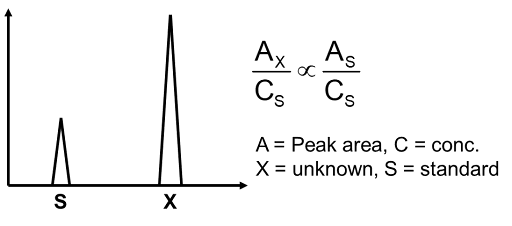
\includegraphics[width=1\textwidth,height=\textheight]{Media/Figure2.png}

}

\caption{\textbf{Figure 2.} Evidence of a changing climate. Adapted from
NASA: Global Climate Change}

\end{figure}

What's concerning is how these changes have severely impacted our
everyday lives. For example, extreme weather events have disrupted the
provision of basic amenities such as water, sanitation and education in
many countries, not to mention the large-scale infrastructure damages
that follow these events. A change in global climate has also negatively
impacted agricultural production and resulted in food security issues.

Under the push for global collaboration on sustainable development, the
United Nations (UN) adopted 17 Sustainable Development Goals (SDG).
\textbf{Goal 13: Climate action} primarily aims to:

\begin{enumerate}
\def\labelenumi{\arabic{enumi}.}
\tightlist
\item
  Improve the resilience and adaptability of all countries to
  climate-related hazards.
\item
  Vitalize initiatives against climate change in national policies and
  planning.
\item
  Emphasize education and develop institutional capacities on climate
  change resilience, adaptability, impact reduction and early warning.
\end{enumerate}

\hypertarget{energy-balance-models-ebms}{%
\subsection{3 \textbar{} ENERGY BALANCE MODELS
(EBMs)}\label{energy-balance-models-ebms}}

In the following chapters, we will understand Earth's climate by
modelling it using Energy Balance Models (EBMs). These models are simple
but very useful to investigate Earth's climate. They do not take into
account the many dynamics of the climate (wind, atmospheric circulation,
ocean currents or convection in oceans or atmosphere) but only focus on
the energetics and thermodynamics of the climate system.

\textbf{Table 1:} Four different EBMs to model Earth's temperature with
increasing complexity
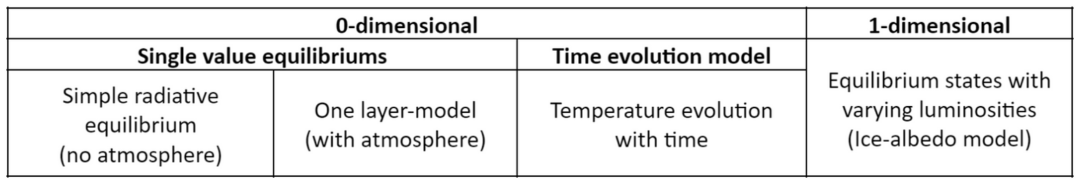
\includegraphics[width=1\textwidth,height=\textheight]{Media/Table1.png}

\hypertarget{simple-radiative-equilibrium-with-no-atmosphere}{%
\subsection{4 \textbar{} SIMPLE RADIATIVE EQUILIBRIUM WITH NO
ATMOSPHERE}\label{simple-radiative-equilibrium-with-no-atmosphere}}

Since Earth's temperature has been stable over a long geological time,
Earth can be perceived to be in a state of radiative equilibrium. It is
a state in which the total thermal radiation received by the object is
equivalent to the total thermal radiation being emitted. In short,
\textbf{the flow of incoming energy = the flow of outgoing energy}
(\textbf{Figure 3}). Using this assumption, we can calculate the
effective temperature of a planet at radiative equilibrium.

\begin{figure}

{\centering 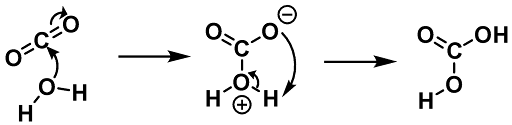
\includegraphics[width=0.8\textwidth,height=\textheight]{Media/Figure3.png}

}

\caption{\textbf{Figure 3.} Incoming solar radiation (left) and outgoing
Earth radiation (right)}

\end{figure}

Although the energy of the geosphere is significant, most of the energy
received on Earth important for life originates from the Sun (Incoming
energy). The received energy then excites atoms and molecules on Earth,
raising the temperature of the corresponding material and results in
thermal infrared energy radiated (Outgoing energy). Let's now have a
look at how we will be calculating the amount of energy received and
emitted by a planet.

\hypertarget{blackbody-radiation}{%
\paragraph{4.1 BLACKBODY RADIATION}\label{blackbody-radiation}}

We can use the concept of blackbody radiation to model the Sun and also
the Earth's flow of energy. A blackbody refers to a model system which
absorbs all incident electromagnetic radiation and for it to remain in
thermal equilibrium, it must emit radiation as well (blackbody
radiation). The blackbody emission spectrum depends on the temperature
of the object and follows \textbf{Planck's law}, \textbf{Wien's law} and
the \textbf{Stefan-Boltzmann law}.

\hypertarget{a-plancks-law}{%
\subparagraph{(A) Planck's Law}\label{a-plancks-law}}

Planck's law shows the electromagnetic spectral distribution of the
radiation coming from a blackbody at a specific temperature in thermal
equilibrium.

\begin{figure}

{\centering 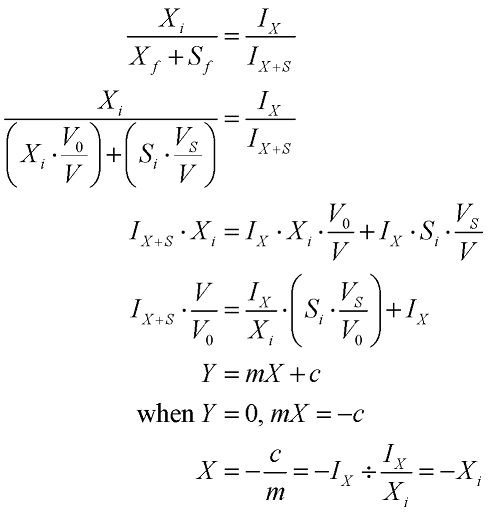
\includegraphics[width=1\textwidth,height=\textheight]{Media/Figure4.png}

}

\caption{\textbf{Figure 4:} (Left) Blackbody emission spectra of an
object with increasing temperature (3000K to 6000K). (Right) Blackbody
emission spectra of the Sun and the Earth}

\end{figure}

\hypertarget{b-wiens-law}{%
\subparagraph{(B) Wien's Law}\label{b-wiens-law}}

Wien's law gives you the relationship between the wavelength of the
maximum emission and the temperature of the blackbody object.

\begin{equation}
\tag{1}
\lambda_{max} = \frac{2898}{T}
\end{equation}

To find the wavelength (\(\lambda_{max}\), \(\mu m\)) of the maximum
emission, divide 2898 by the temperature (\(T\),\(K\)).

\hypertarget{c-stefan-boltzmann-law}{%
\subparagraph{(C) Stefan-Boltzmann Law}\label{c-stefan-boltzmann-law}}

The Stefan-Boltzmann Law gives you the flux of energy (the rate of
transfer of energy per unit area) emitted by the blackbody object
(\(F\)) at a specific temperature (for a perfect blackbody we have):

\begin{equation}
\tag{2}
F = \sigma T^{4}
\end{equation}

The flux (\(F\), \(W m^{-2}\)) emitted is the product of the temperature
(\(T\), \(K\)) of the blackbody and the Stefan-Boltzmann constant
(\(\sigma = 5.67 * 10^{-8} W m^{-2} K^{-4}\)).

\hypertarget{d-calculation-of-flux-received-at-the-surface-of-a-planet}{%
\subparagraph{(D) Calculation of flux received at the surface of a
planet}\label{d-calculation-of-flux-received-at-the-surface-of-a-planet}}

To calculate the amount of flux received on the surface of a planet from
the star \(S_{0}\), we have to utilise the inverse square law
(\textbf{Figure 5}). It says that the energy density is inversely
proportional to the square of the distance from the source, while the
total energy emitted from the source is constant.

\begin{figure}

{\centering 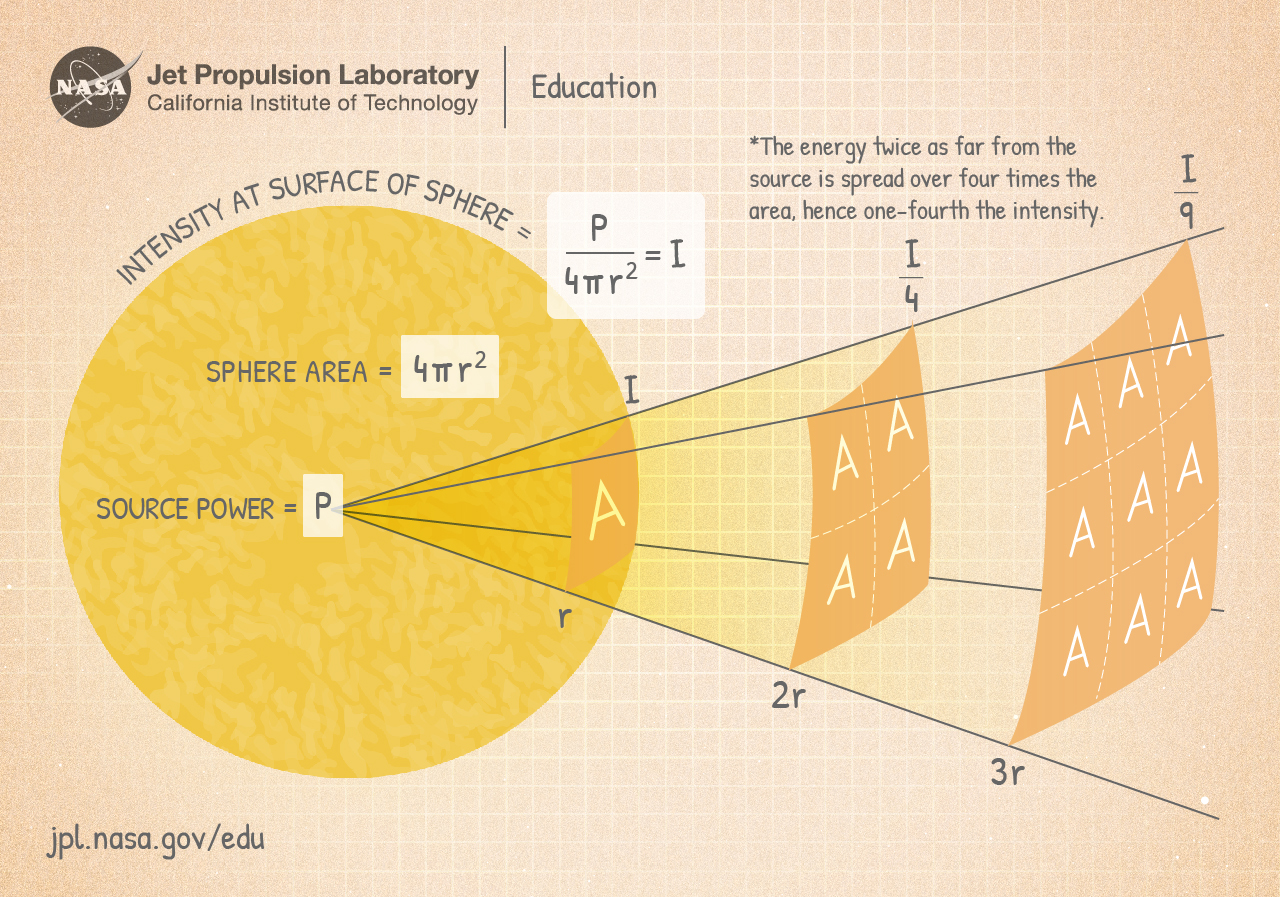
\includegraphics[width=0.8\textwidth,height=\textheight]{Media/Figure5.jpg}

}

\caption{\textbf{Figure 5:} Illustration of energy dispersion through
the inverse square law.}

\end{figure}

\begin{equation}
\tag{3}
\frac{F}{S_{0}} = \frac{R_{p}^{2}}{r_{s}^{2}}
\end{equation}

The ratio between the flux emitted from the surface of the sun (\(F\),
\(W m^{-2}\)) and the flux received on a planet (\(S_{0}\),
\(W m^{-2}\)) equals the ratio between the square of the planet's
distance from the sun (\(R_{p}\), \(m\)) and the square of the Sun's
radius (\(r_{s}\), \(m\)).

\hypertarget{albedo}{%
\paragraph{4.2 ALBEDO}\label{albedo}}

Not all the light from the Sun is received by a planet, with one part
being reflected off. The amount reflected depends on the albedo of the
surface \(\alpha\) (\textbf{Table 2}).

\begin{equation}
\tag{4}
S_0' = S_0\alpha
\end{equation}

The flux reflected by the planet (\(S_0'\), \(W m^{-2}\)) is the product
of the flux received by the planet (\(S_0\), \(W m^{-2}\)) and its
albedo (\(\alpha\)).

\textbf{Table 2:} Albedo of various surfaces

\begin{figure}

{\centering 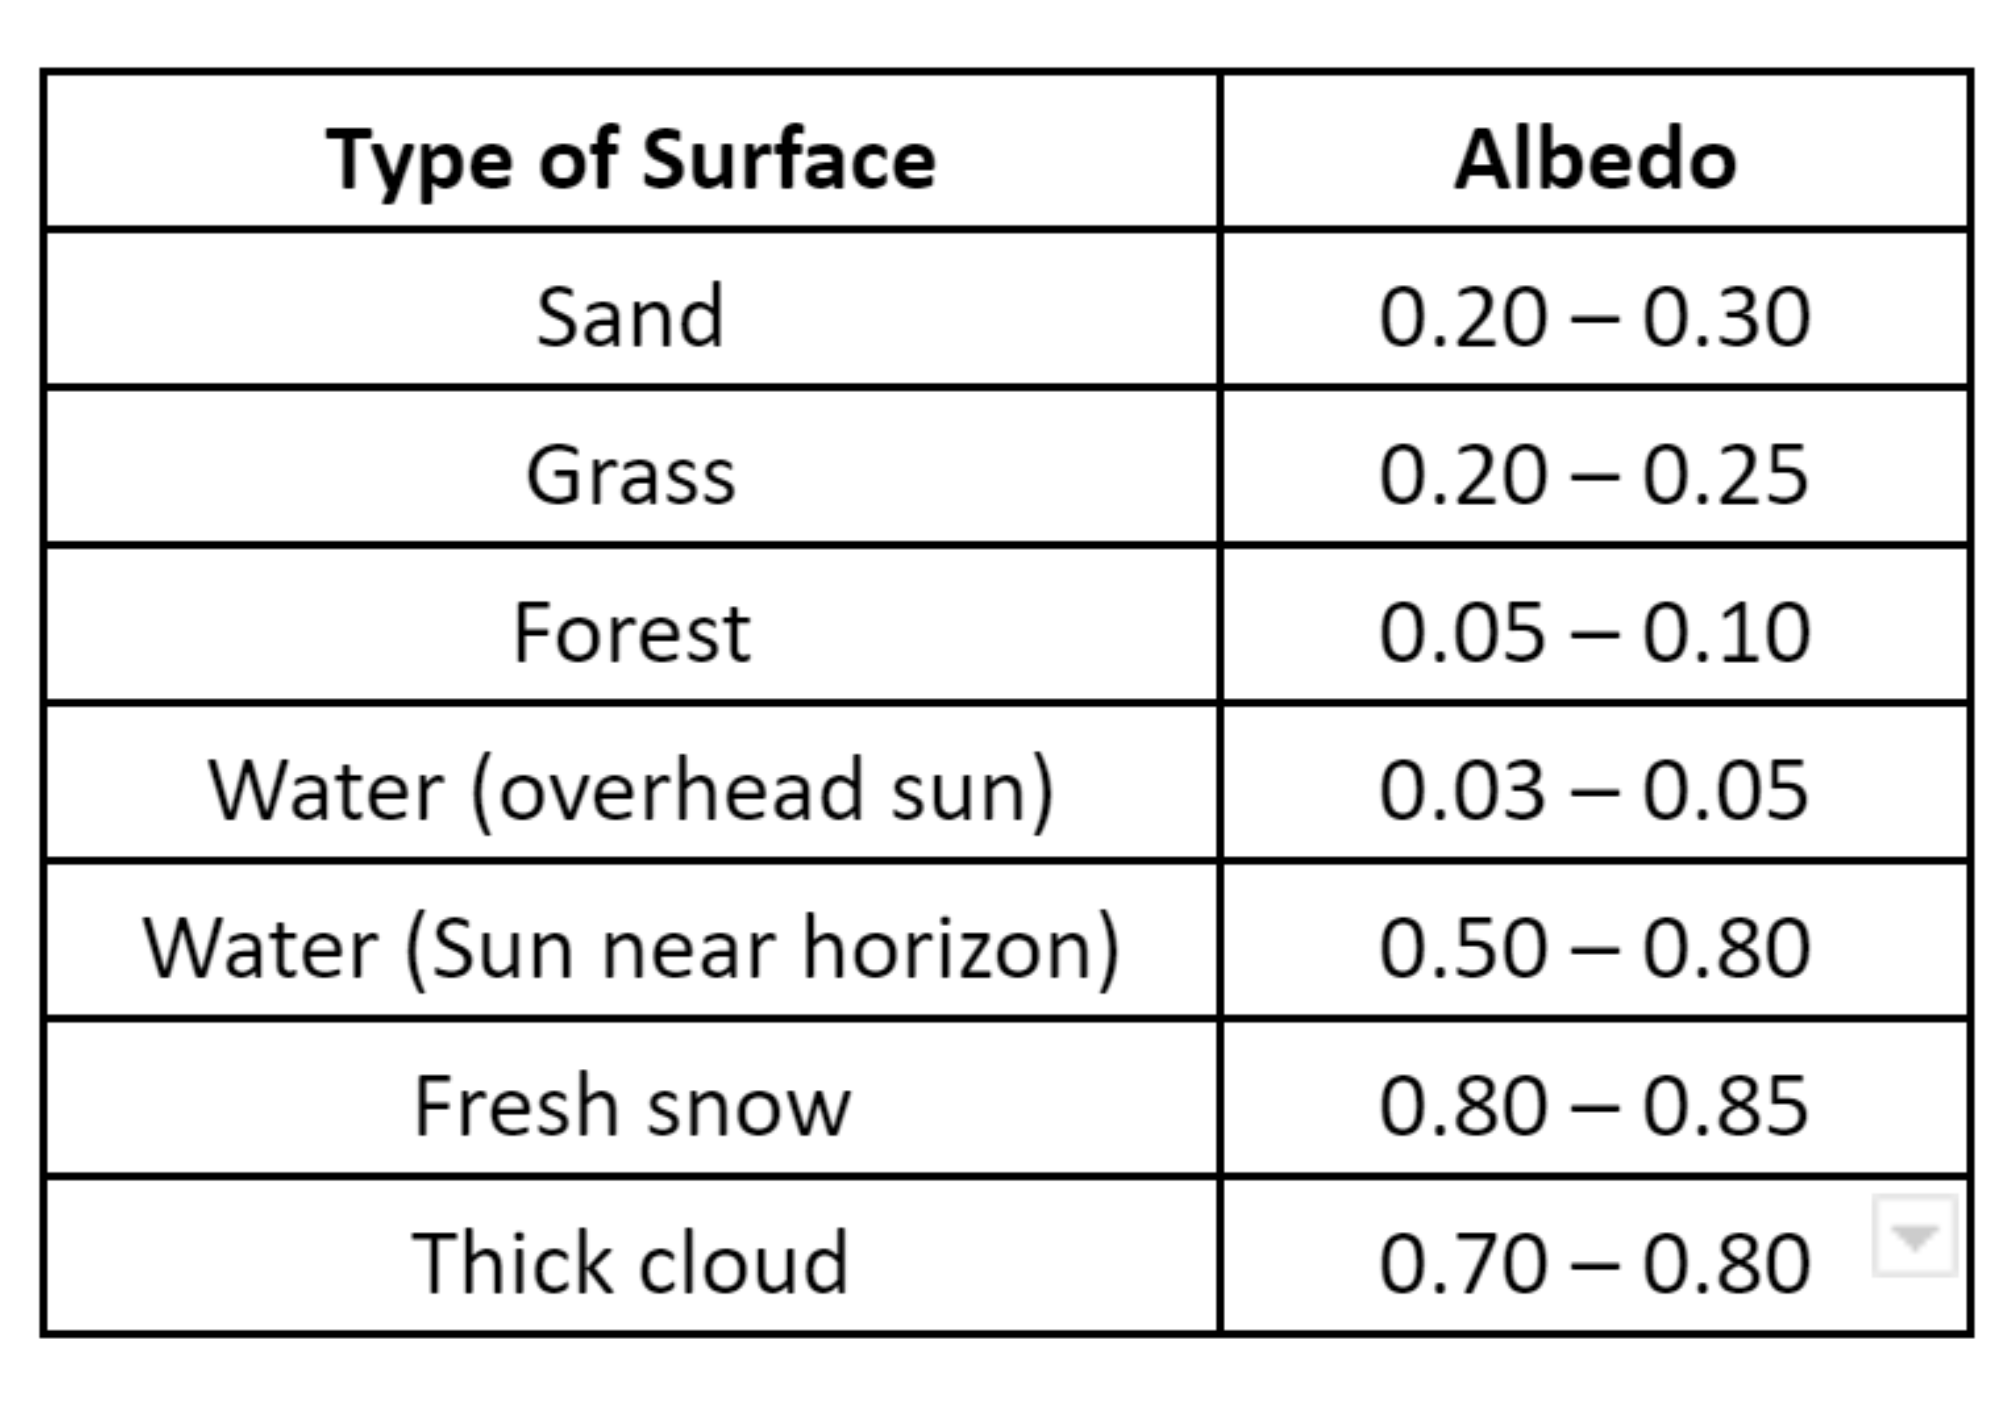
\includegraphics[width=0.5\textwidth,height=\textheight]{Media/Table2.png}

}

\end{figure}

\hypertarget{effective-temperature-of-a-planet}{%
\paragraph{4.3 EFFECTIVE TEMPERATURE OF A
PLANET}\label{effective-temperature-of-a-planet}}

We are now able to calculate the effective temperature of a planet at
radiative equilibrium. The planet absorbs the energy from the Sun (Solar
flux, \(S_0\)) and emits radiation as a blackbody (Planet flux,
\(F_p\)). The albedo (\(\alpha\)) is the fraction of light being
reflected.

To convert flux to energy, we have to multiply it by its effective
surface area (\textbf{Figure 6}). A planet intercepts incoming solar
flux with its cross-sectional area \(\pi R^2\). However, the planet flux
is emitted over the entire spherical surface area of the planet of
4\(\pi R^2\).

\begin{figure}

{\centering 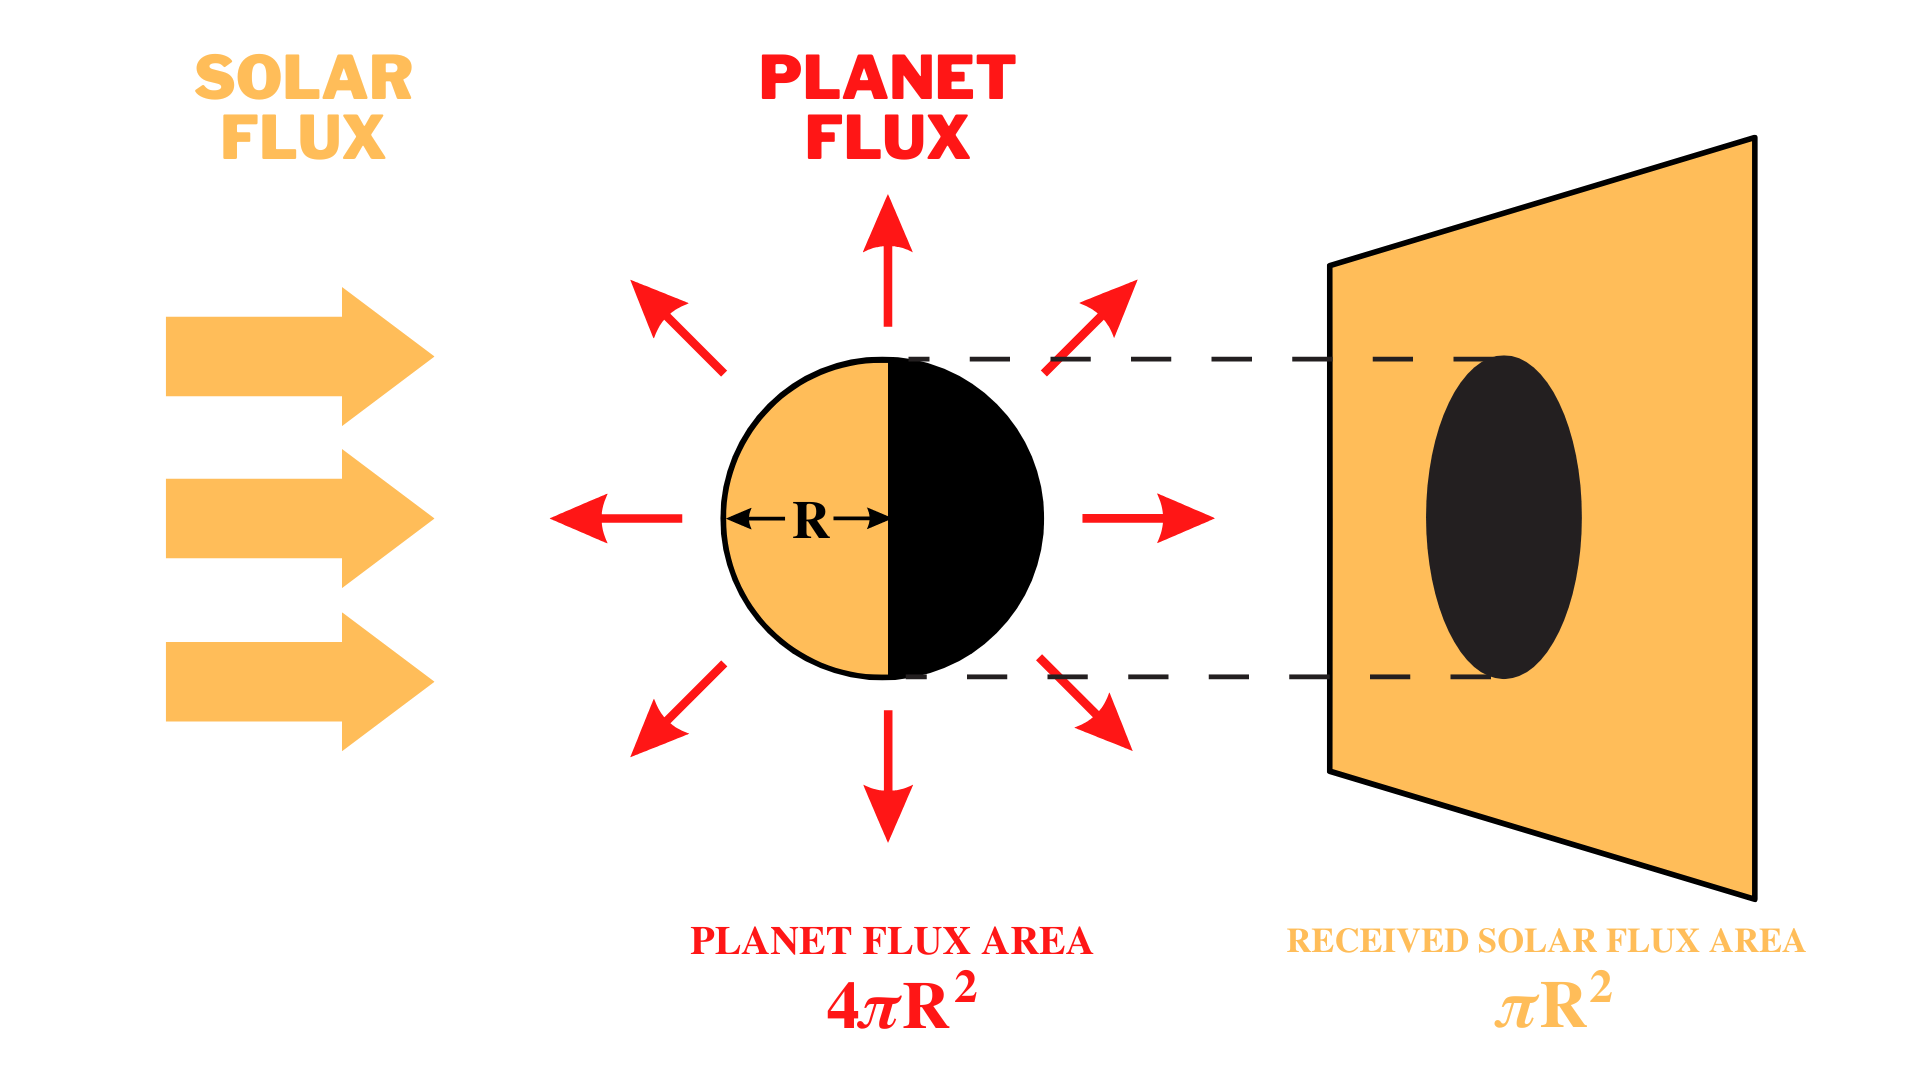
\includegraphics[width=0.5\textwidth,height=\textheight]{Media/Figure6.png}

}

\caption{\textbf{Figure 6:} The effective surface areas of incoming
solar flux and the planet flux}

\end{figure}

We can then derive the equation for a planet's temperature at energy
balance equilibrium to be:

\begin{equation}
\tag{5}
T_{p} = \sqrt[4]{\frac{S_0(1-\alpha)}{4\sigma}}
\end{equation}

\subsubsection{\texorpdfstring{\textbf{Exercise 1}}{Exercise 1}}

Derive the equation for a planet's temperature at energy balance
equilibrium: \[T_{p} = \sqrt[4]{\frac{S_0(1-\alpha)}{4\sigma}}\]

\textbf{Hint:} Start from \(E_{absorbed} = E_{emitted}\)

\subsubsection{\texorpdfstring{\textbf{Model Answer}}{Model Answer}}

\[E_{absorbed} = E_{emitted}\]
\[E_{received} - E_{reflected} = E_{emitted}\]

\(S_0\) \(*\) area of cross-section - \(S_0\) \(*\) \(\alpha\) \(*\)
area of cross-section = \(F_p\) \(*\) Planet's surface area

\[S_0 * \pi r_p^2 * (1 - \alpha) = \sigma T_p^4 * 4 \pi r_p^2\]
\[T_{p} = \sqrt[4]{\frac{S_0(1-\alpha)}{4\sigma}}\]

\begin{tcolorbox}[enhanced jigsaw, titlerule=0mm, title={Modelling Questions}, arc=.35mm, breakable, colback=white, toprule=.15mm, colframe=quarto-callout-caution-color-frame, opacityback=0, bottomtitle=1mm, coltitle=black, toptitle=1mm, rightrule=.15mm, colbacktitle=quarto-callout-caution-color!10!white, bottomrule=.15mm, opacitybacktitle=0.6, leftrule=.75mm, left=2mm]

\textbf{M1.} Write code to calculate the flux received on a planet
(\(S_0\)) given the following parameters: \textbf{1.} Temperature of the
star (Sun), \(T_s\) = \(5780\) K \textbf{2.} Radius of the star (Sun),
\(r_s\) = \(6.96 * 10^8 m\) \textbf{3.} Distance of the planet (Earth)
from the star (Sun), \(R_p\) = 1 AU \textbf{Hint:} Use Stefan-Boltzmann
Law (2) and the Inverse square law (3).

\begin{center}\rule{0.5\linewidth}{0.5pt}\end{center}

\textbf{M2.} Using \(S_0\) from \textbf{M1}, calculate the effective
temperature of the planet (Earth) at radiative equilibrium given an
albedo (\(\alpha\)) of 0.3.

\begin{center}\rule{0.5\linewidth}{0.5pt}\end{center}

\textbf{M3.} Using the code you constructed, calculate the effective
temperatures of \textbf{Venus}, \textbf{Earth} and \textbf{Mars} using
the parameters below (albedo and distance from the Sun). Are the
simulated temperatures the same as the experimentally measured
temperatures?\textbf{Venus}Albedo = 0.8, Distance from the Sun (AU) =
0.72, Measured temperature (K) = 730\textbf{Earth}Albedo = 0.3, Distance
from the Sun (AU) = 1, Measured temperature (K) = 288\textbf{Mars}Albedo
= 0.22, Distance from the Sun (AU) = 1.52, Measured temperature (K) =
218

\end{tcolorbox}

\hypertarget{one-layer-model}{%
\subsection{5 \textbar{} ONE-LAYER MODEL}\label{one-layer-model}}

\hypertarget{greenhouse-gases}{%
\paragraph{5.1 GREENHOUSE GASES}\label{greenhouse-gases}}

From the results of \textbf{M3}, a difference between the temperature
modelled using your code and the actual temperature measured can be
observed. This is because the simple radiative equilibrium model does
not take planetary atmosphere into consideration. Although present in
very small amounts in the atmosphere, some gases have a great impact on
Earth's temperature. They are called greenhouse gases.

The greenhouse effect is the trapping of infra-red radiation by gases,
resulting in an increase of the surface temperature. Infra-red active
molecules show a change in their dipole moment (permanent dipole is not
necessary) during vibration as seen in \textbf{Figure 7}.

\begin{figure}

{\centering 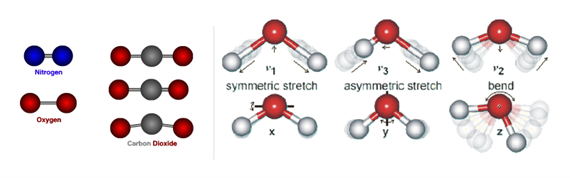
\includegraphics[width=0.8\textwidth,height=\textheight]{Media/Figure7.png}

}

\caption{\textbf{Figure 7:} Molecular vibrations of N2, O2, CO2 and H2O.
You can view the animations
\href{https://scied.ucar.edu/learning-zone/atmosphere/molecular-vibration-modes}{here}.}

\end{figure}

Greenhouse gases absorb the infra-red radiation emitted by the solid
Earth and re-emit them back into the atmosphere. \textbf{Figure 8} shows
how much infra-red radiation emitted from the Earth is re-absorbed by
the atmosphere. In particular, we can take note of the absorption bands
of water and carbon dioxide.

\begin{figure}

{\centering 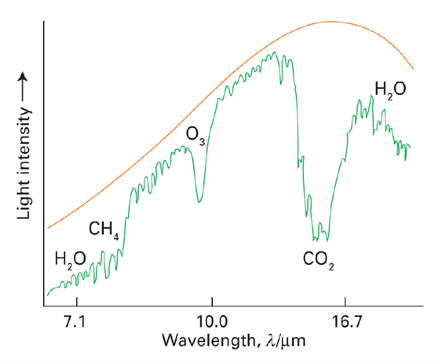
\includegraphics[width=0.6\textwidth,height=\textheight]{Media/Figure8.png}

}

\caption{\textbf{Figure 8:} The amount of greenhouse gas IR-absorption
is shown in green and the Earth blackbody emitted radiation is shown in
orange.}

\end{figure}

For \textbf{M3}, Venus has a thick atmosphere that is primarily
comprised of CO2 (around 96.5\%). Hence, its strong greenhouse effect on
Venus retains more heat in its atmosphere, resulting in the observed
large temperature increment. In contrast, while Mars also has a
predominantly CO2 atmosphere (around 95.32\%), its atmosphere is really
thin, and thus plays a relatively weak role in retaining heat. As such,
the previous model can provide a close approximation to Mars'
temperature.

\hypertarget{one-layer-model-1}{%
\paragraph{5.2 ONE-LAYER MODEL}\label{one-layer-model-1}}

The one-layer model is a simple model to show the effect of the
atmosphere on a planet's temperature. \textbf{Figure 9} shows the solar
radiation \(F_s\) entering the atmosphere and only a fraction \(\tau_s\)
goes through and reaches the planet's surface. Similarly, the flux
emitted by the planet surface \(F_g\) comes out of the layer of
atmosphere with a fraction \(\tau_g\). The values for \(\tau_s\) and
\(\tau_g\) are 0.8 and 0.1 respectively on Earth. Finally, \(F_a\)
represents the radiation emitted by the atmosphere (also modelled as a
blackbody).

\begin{figure}

{\centering 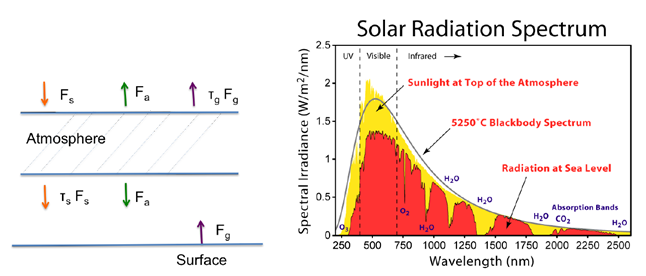
\includegraphics[width=1\textwidth,height=\textheight]{Media/Figure9.png}

}

\caption{\textbf{Figure 9:} \textbf{Left}, One-layer model: \(F_s\),
\(F_g\) and \(F_a\) are respectively the emission from the sun, the
Earth's surface and the atmosphere (with \(\tau_s\) = 0.8 and \(\tau_g\)
= 0.1). \textbf{Right}, The blackbody emission spectrum of the sun and
measured solar radiation before and after going through the atmosphere.}

\end{figure}

\subsubsection{\texorpdfstring{\textbf{Exercise 2}}{Exercise 2}}

What does \(\tau_s\) and \(\tau_g\) represent? Explain the difference in
value.

\subsubsection{\texorpdfstring{\textbf{Model Answer}}{Model Answer}}

\(\tau_s\) represents the fraction of solar flux going through the
atmosphere. As the primary wavelengths of incoming solar energy is in
the visible spectrum, and the atmosphere is not opaque to visible light,
most of the solar flux is able to pass through, resulting in a high
value of 0.8.

On the contrary, \(\tau_g\) represents the fraction of planet flux
passing through the atmosphere into space. As the primary emissions are
in the infra-red range allowing for greenhouse gas IR-absorption, not
much of the emissions goes through the atmosphere, resulting in a low
value of 0.1.

\subsubsection{\texorpdfstring{\textbf{Exercise 3}}{Exercise 3}}

Assume there is a radiative equilibrium both at the top of the
atmosphere and at the surface of the Earth (bottom of the atmosphere),
derive an expression for the flux emitted from the ground (\(F_g\)) as a
function of \(F_s\), \(\tau_s\), \(\tau_g\) (see \textbf{Figure 9})

\subsubsection{\texorpdfstring{\textbf{Model Answer}}{Model Answer}}

At the top of the atmosphere:

\[F_s = F_a + F_g\tau_g\] \[F_a = F_s - F_g\tau_g\] At the bottom of the
atmosphere:

\[F_s\tau_s + F_a = F_g\] \[F_a = F_g - F_s\tau_s\] Combining (1) and
(2):

\[F_s - F_g\tau_g = F_g - F_s\tau_s\] \[F_s(1+\tau_s) = F_g(1+\tau_g)\]
\[F_g = F_s\frac{(1+\tau_s)}{(1+\tau_g)}\]

\subsubsection{\texorpdfstring{\textbf{Exercise 4}}{Exercise 4}}

From the previous simplified equation in \textbf{Exercise 3}, derive the
equation to calculate the effective temperature of the planet (\(T_p\))
with an atmosphere.

\subsubsection{\texorpdfstring{\textbf{Model Answer}}{Model Answer}}

\[F_g = F_s\frac{(1+\tau_s)}{(1+\tau_g)}\]
\[\sigma T^4 * 4\pi R^2 = \frac{S_0 * \pi R^2 * (1-\alpha)*(1+\tau_s)}{(1+\tau_g)}\]
\[T = \sqrt[4]{\frac{S_0 * (1-\alpha)*(1+\tau_s)}{4\sigma(1+\tau_g)}}\]

\begin{tcolorbox}[enhanced jigsaw, titlerule=0mm, title={Modelling Questions}, arc=.35mm, breakable, colback=white, toprule=.15mm, colframe=quarto-callout-caution-color-frame, opacityback=0, bottomtitle=1mm, coltitle=black, toptitle=1mm, rightrule=.15mm, colbacktitle=quarto-callout-caution-color!10!white, bottomrule=.15mm, opacitybacktitle=0.6, leftrule=.75mm, left=2mm]

\textbf{M4.} Construct a code and calculate the effective temperature of
Earth with a simulated atmosphere of \(\tau_s\) = 0.8 and \(\tau_g\) =
0.1.

\end{tcolorbox}

\hypertarget{temperature-evolution-model}{%
\subsection{6 \textbar{} TEMPERATURE EVOLUTION
MODEL}\label{temperature-evolution-model}}

\hypertarget{earth-as-a-greybody}{%
\paragraph{6.1 EARTH AS A GREYBODY}\label{earth-as-a-greybody}}

So far, we have modelled the planet as a perfect blackbody and therefore
the emitted flux Fg (\(W m^{-2}\)):

\begin{equation}
F_{g} = \epsilon\sigma * T^4 = \sigma * T^4
\end{equation}

\(\epsilon\) is the emissivity of the body. It varies from 0 (no
emission) to 1 (perfect blackbody emission). A body with an emissivity
less than 1 is called a greybody.

From the one-layer model, we see that the atmosphere affects a planet's
surface temperature greatly through the introduction of \(\tau\).
Comparing it to the simple radiative equilibrium model which assumes the
Earth as a perfect blackbody (\(\epsilon\) = 1), we can find that it
does not model well the real surface temperature.

In essence, due to the insulative blanket that the atmosphere causes,
the emitted flux back to space will be lower. Hence, the emissivity of
the body is lower and the surface temperature will be higher. By
including the coefficient \(\epsilon\), we can model better the real
surface temperature. Note we cannot directly measure \(\epsilon\), but
we can adjust the value according to temperature and flux observations.

\hypertarget{temperature-linearisation}{%
\paragraph{6.2 TEMPERATURE
LINEARISATION}\label{temperature-linearisation}}

In order to make the modelling easier, we'll be doing temperature
linearisation (possible because \(T_c\) = \(\pm\) 20\(^\circ\)C).
Sellers (1969) and Budyko (1969) in the 60's demonstrated that Earth's
energy emission could be written in a linear form with the temperature.
Much later, it was proven to fit very well with energy flux
observations.

Since for small \(x\), we can write \((1+x)^4 \approx 1 + 4x\)

\[T_K^4 = (T_0 + T_c)^4 = T_0^4 * (1 + \frac{T_c}{T_0})^4 \approx T_0^4 * (1+4\frac{T_c}{T_0})\]
The temperature in Kelvin (\(T_K\)), the 0\(^\circ\)C in Kelvin (\(T_0\)
= 273.15K) and temperature in Celcius (\(T_c\))

\[{T_K}^4 = {T_0}^4 + 4{T_0}^3 * T_c = a + bT_c\]

As \(a\) and \(b\) are constants, we can simplify:

\begin{equation}
\tag{6}
F_g = \epsilon\sigma * {T_K}^4 = \epsilon\sigma(a + bT_c) = A + BT_c
\end{equation}

With A (\(W m^{-2}\)) and B (\(W m^{-2}\) \(^\circ C\)) constants. A and
B reflect the \textbf{emissivity} of the atmosphere. They will be given
and they vary with the type of atmosphere (amount of greenhouse gases).
More or less, the constants A and B can tell us the following:

\textbf{Table 3:} Representation of the constants A and B

\begin{figure}

{\centering 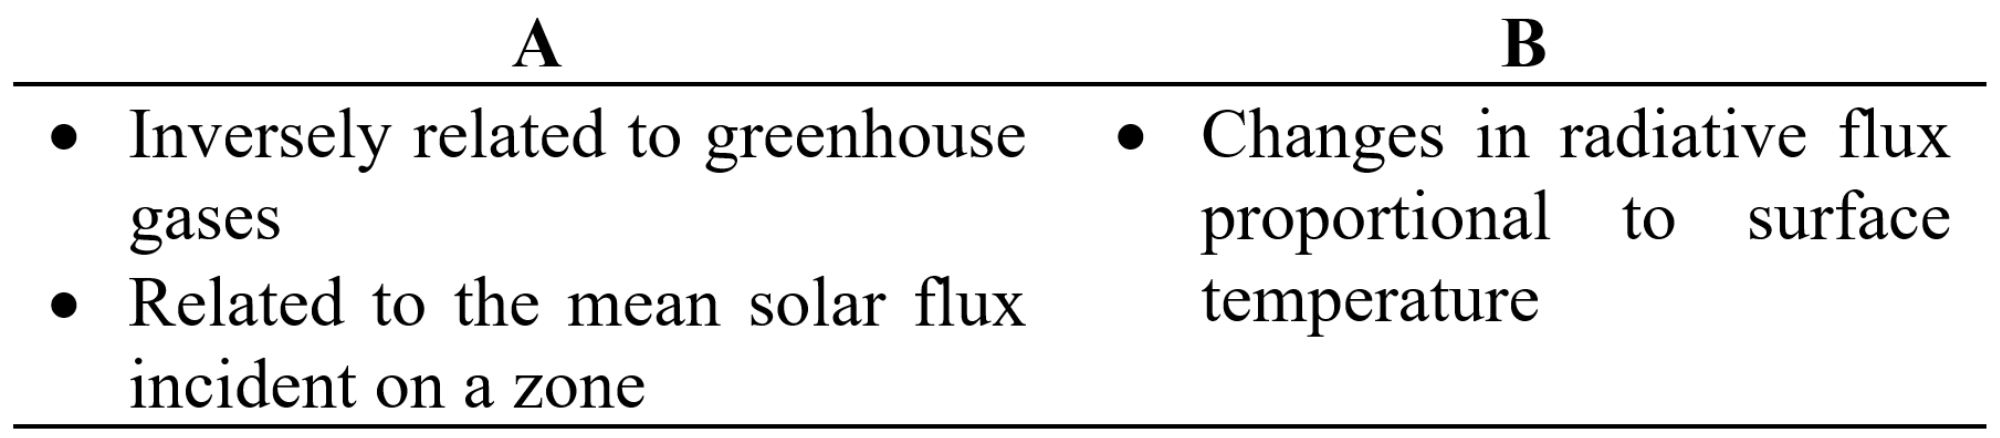
\includegraphics[width=0.7\textwidth,height=\textheight]{Media/Table3.png}

}

\end{figure}

You can find in \textbf{Table 4}, different values reported in
literature.

\textbf{Table 4:} Values of A and B reported in literature

\begin{figure}

{\centering 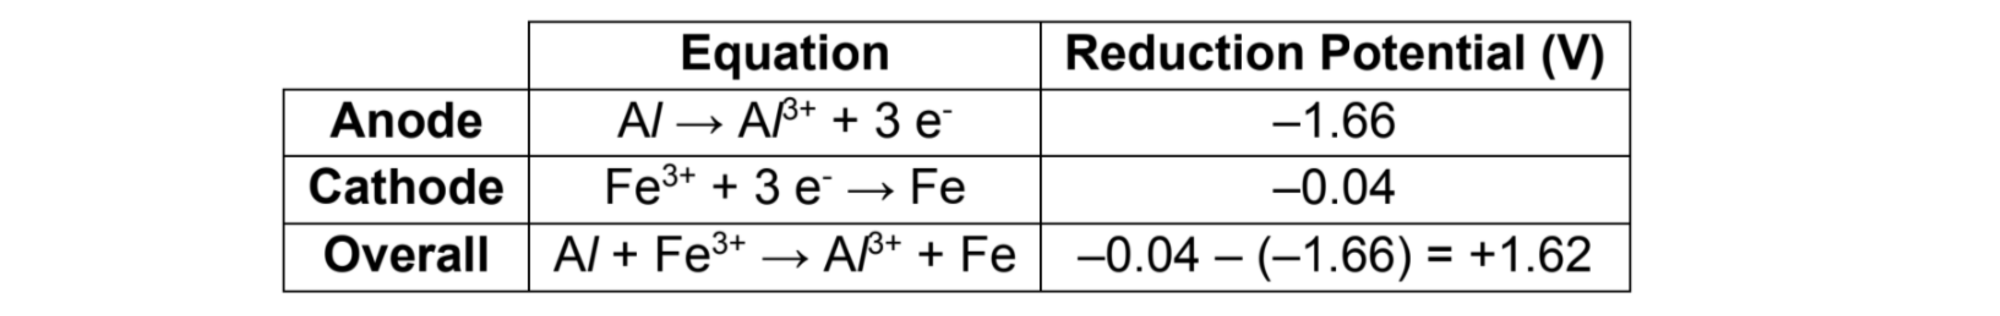
\includegraphics[width=0.7\textwidth,height=\textheight]{Media/Table4.png}

}

\end{figure}

\begin{tcolorbox}[enhanced jigsaw, titlerule=0mm, title={Modelling Questions}, arc=.35mm, breakable, colback=white, toprule=.15mm, colframe=quarto-callout-caution-color-frame, opacityback=0, bottomtitle=1mm, coltitle=black, toptitle=1mm, rightrule=.15mm, colbacktitle=quarto-callout-caution-color!10!white, bottomrule=.15mm, opacitybacktitle=0.6, leftrule=.75mm, left=2mm]

\textbf{M5.} Recalling what the linearisation constants (A and B) stand
for, translate the equations into code and calculate the temperature of
Earth using the constants from McGuffie (2005).

\end{tcolorbox}

\hypertarget{temperature-evolution-model-1}{%
\paragraph{6.3 TEMPERATURE EVOLUTION
MODEL}\label{temperature-evolution-model-1}}

In this model, we are interested to find the change of temperature with
time and find the equilibrium temperature of the planet as it reaches
radiative equilibrium. We will be modelling Earth's emission as written
in \emph{5.2} using the values for a greybody. Thus, the equations for
Earth's average energy gain (\(E_{gain}\)) and energy loss
(\(E_{loss}\)) for this model would be:

\[E_{gain} = S_0* (1-\alpha)*\pi r^2\]
\[E_{loss} = (A + BT_c) * 4\pi r^2\] Removing the common terms and
divide both terms by 4, we'll get:

\[E_{gain} = \frac{S_0* (1-\alpha)}{4}\] \[E_{loss} = A + BT_c\]

The absorption of heat of a body is controlled by the heat capacity (C).
So, the difference between the energy gain and the energy loss of the
Earth can be expressed:

\begin{equation}
\tag{7}
C * \frac{dT}{dt} = E_{gain} - E_{loss}
\end{equation}

The rate of heat flow (\(\frac{dT}{dt}\)) is proportional to the
difference between the energy gained and energy loss by Earth.

\begin{tcolorbox}[enhanced jigsaw, titlerule=0mm, title={Modelling Questions}, arc=.35mm, breakable, colback=white, toprule=.15mm, colframe=quarto-callout-caution-color-frame, opacityback=0, bottomtitle=1mm, coltitle=black, toptitle=1mm, rightrule=.15mm, colbacktitle=quarto-callout-caution-color!10!white, bottomrule=.15mm, opacitybacktitle=0.6, leftrule=.75mm, left=2mm]

Let's construct a code for a temperature evolution model that simulates
how Earth's temperature slowly equilibrates over time.

\textbf{M6.} Calculate Earth's Heat Capacity (\(C\)) based on Earth's
water content. Given:\\
Depth of water: \(70\) m Density of water: \(1.025 * 10^6\) g/m\(^3\)
Heat capacity of water: \(4.186\) J/g\(*\)K Ocean coverage: \(0.7\)

\begin{center}\rule{0.5\linewidth}{0.5pt}\end{center}

\textbf{M7.} Calculate Earth's average \(E_{gain}\) (Energy gain in
Watts/m\(^2\)). Given:\\
\(S_0\): 1370 Watts/m\(^2\) Albedo: 0.32

\begin{center}\rule{0.5\linewidth}{0.5pt}\end{center}

\textbf{M8.} Based on the final equation from \textbf{5.3}, use the
Euler method to simulate Earth's temperature slowly equilibrating over
time from a given initial temperature. After each iteration, store the
temperature (\textbf{T}) and the time (\textbf{t}) in a list to be
plotted at the end.

\begin{figure}[H]

{\centering 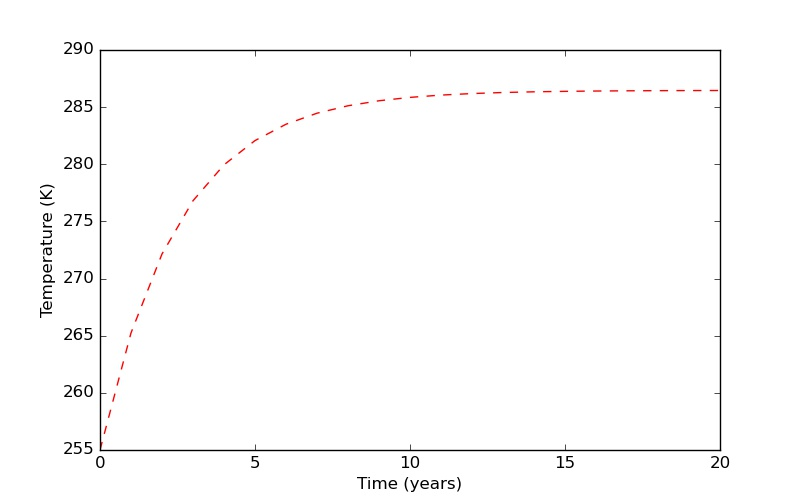
\includegraphics[width=0.8\textwidth,height=\textheight]{Media/Plot1.jpg}

}

\end{figure}

Here are some variables you can consider initializing at the start of
the model: \emph{Count}: To keep track of the number of loops
\emph{Starting temperature} (T\_0): 255 K \emph{Starting time} (t\_0): 0
seconds \emph{Timestep or dt}: 1 Year or 31536000 seconds Two lists to
store the time and temperature from each iteration

You may use the below flowchart to assist in your coding of the
iteration loop.
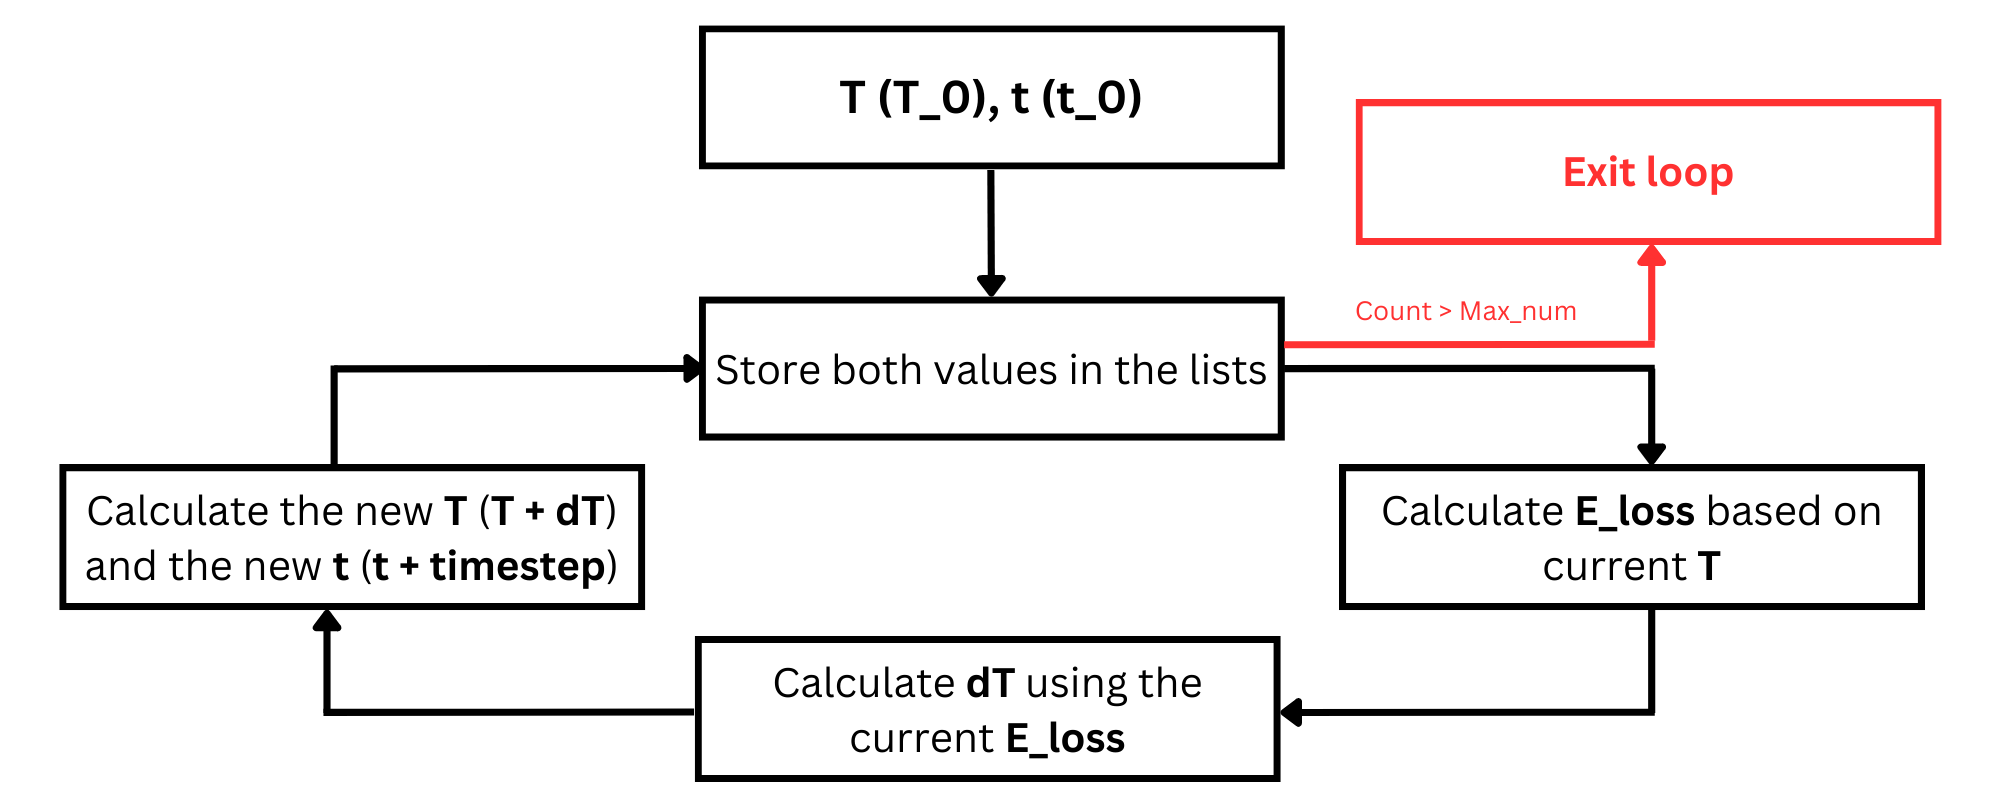
\includegraphics[width=1\textwidth,height=\textheight]{Media/FlowChart1.png}

Finally, plot the data obtained.

\end{tcolorbox}

\hypertarget{the-push-over-the-edge}{%
\subsection{7 \textbar{} THE PUSH OVER THE
EDGE}\label{the-push-over-the-edge}}

\hypertarget{tipping-points}{%
\paragraph{7.1 TIPPING POINTS}\label{tipping-points}}

In a climate system, tipping points are what climatologists refer to as
vulnerable areas that when triggered, could result in a climate
emergency with irreversible consequences (Lenton et al., 2019). Examples
of tipping points often being discussed include the melting of the
arctic sea ice, deforestation in the Amazon basin and widescale coral
bleaching events. Following the recent trend of global warming,
climatologists are now concerned of the risk of a cascade of tipping
points crossing their critical thresholds, leading to severe
repercussions on the climate, our ecosystems and our societies
(Wunderling et al., 2021).

\begin{figure}

{\centering \includegraphics[width=0.8\textwidth,height=\textheight]{Climate_files/mediabag/raising-the-alarm-cl.jpg}

}

\caption{\textbf{Figure 10:} Significant tipping points hypothesized and
the cascading connections between them.}

\end{figure}

\hypertarget{feedback-loops}{%
\paragraph{7.2 FEEDBACK LOOPS}\label{feedback-loops}}

To understand climate tipping points, let's first try to imagine how
Earth's climate would be like given the following situations:

\subsubsection{\texorpdfstring{\textbf{Exercise 5}}{Exercise 5}}

What would happen to the Earth if it experiences an extreme increase of
solar insolation? Predict the changes using the water vapor feedback
mechanism (\textbf{Figure 11}). Explain the mechanism of this feedback.
Does it happen easily? Why?\\
(Think of the relationship between pressure and the boiling point,
\textbf{Figure 12})

\begin{figure}

{\centering 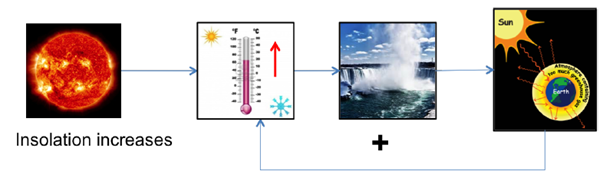
\includegraphics[width=1\textwidth,height=\textheight]{Media/Figure11.png}

}

\caption{\textbf{Figure 11:} Water vapor feedback.}

\end{figure}

\begin{figure}

{\centering 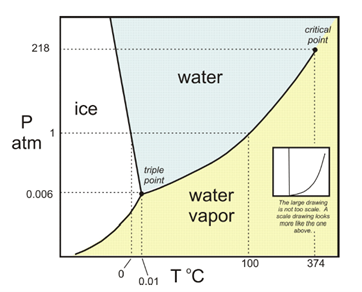
\includegraphics[width=0.5\textwidth,height=\textheight]{Media/Figure12.png}

}

\caption{\textbf{Figure 12:} The phase diagram of water.}

\end{figure}

\subsubsection{\texorpdfstring{\textbf{Model Answer}}{Model Answer}}

From the water vapor feedback mechanism, when Earth experiences an
extreme increase of solar insolation, the temperature on Earth would
increase, causing more water evaporation to occur on Earth. As water
vapor is a greenhouse gas, it would result in the further retainment of
heat in the atmosphere, leading to increasing temperatures on Earth.
Hence, it is viewed as a positive feedback loop.

However, it doesn't happen easily as when there is an increase of water
vapor in the air, it results in a higher atmospheric pressure which
increases the boiling point of water. As such, the amount of evaporation
would reduce. This counter-mechanism helps mediate the water vapor
feedback.

\subsubsection{\texorpdfstring{\textbf{Exercise 6}}{Exercise 6}}

What would happen to the Earth if it experiences an extreme decrease in
solar insolation? Predict the changes using the Ice-albedo feedback
mechanism (\textbf{Figure 13}). Explain the mechanism of this feedback.

\begin{figure}

{\centering 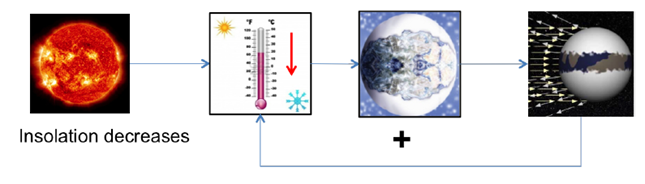
\includegraphics[width=1\textwidth,height=\textheight]{Media/Figure13.png}

}

\caption{\textbf{Figure 13:} Ice-albedo feedback.}

\end{figure}

\subsubsection{\texorpdfstring{\textbf{Model Answer}}{Model Answer}}

Following the ice-albedo feedback loop, if Earth experiences an extreme
decrease in solar insolation, Earth's temperature would reduce. As a
result, the ice caps would extend to lower latitudes from the poles. An
increase in polar ice caps results in an increase in planetary albedo,
which leads to a reduced amount of energy entering Earth's climate
system. This then further causes a reduction in temperature, completing
the positive feedback loop.

\begin{quote}
\textbf{Discussion corner}

Can you relate the above two scenarios (Water vapor feedback \&
Ice-albedo feedback) with Earth or other planets? Explain.
\end{quote}

\hypertarget{the-ice-albedo-model}{%
\subsection{8 \textbar{} THE ICE-ALBEDO
MODEL}\label{the-ice-albedo-model}}

\hypertarget{model-description}{%
\paragraph{8.1 MODEL DESCRIPTION}\label{model-description}}

In this final climate model, we will compute the equilibrium
temperatures of the Earth following the Ice-albedo model when:

\begin{enumerate}
\def\labelenumi{\arabic{enumi}.}
\tightlist
\item
  The solar luminosity is increasing
\item
  The solar luminosity is decreasing
\item
  Ice is forming
\end{enumerate}

In our previous models, we have kept the albedo of the planet constant.
Now, we will vary the albedo of the planet through the simulation of ice
forming on the planet, which in turn is affected by the temperature.

This model takes into account the contribution of each latitude (surface
area and local temperature) to calculate the average temperature of
Earth.

The objectives are:

\begin{enumerate}
\def\labelenumi{\arabic{enumi}.}
\tightlist
\item
  Generate the temperature data for a range of solar radiation
  (\emph{luminosity}).
\item
  Plot the graph T (\emph{temperature}) against M (\emph{solar
  multiplier})
\end{enumerate}

\begin{figure}

{\centering \includegraphics[width=1\textwidth,height=\textheight]{Media/Icealbedo.gif}

}

\caption{\textbf{Figure 14:} Ice-albedo model illustration when solar
luminosity is decreasing.}

\end{figure}

\hypertarget{model-set-up}{%
\paragraph{8.2 MODEL SET-UP}\label{model-set-up}}

\hypertarget{a-energy-gain}{%
\subparagraph{(A) Energy gain}\label{a-energy-gain}}

\begin{figure}

{\centering 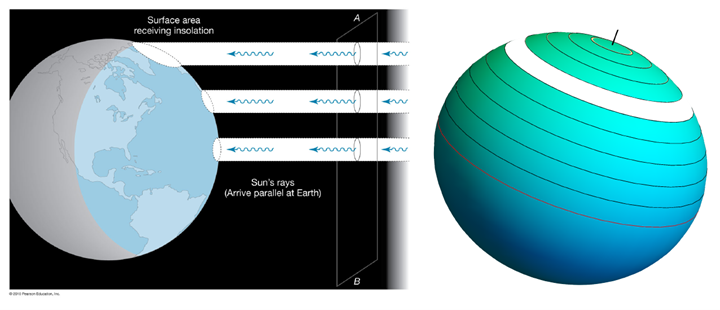
\includegraphics[width=1\textwidth,height=\textheight]{Media/Figure14.png}

}

\caption{\textbf{Figure 15:} Distribution of the solar flux across
latitudes.}

\end{figure}

We divide the hemisphere in 10 bands of 9\(^\circ\) latitude each
(\textbf{Figure 14}). The area of each band (in fraction) and the local
solar flux (\(S_i\)) is reported in \textbf{Table 5}.

\textbf{Table 5:} Area and local solar flux received for each latitude
bands.

\begin{figure}

{\centering 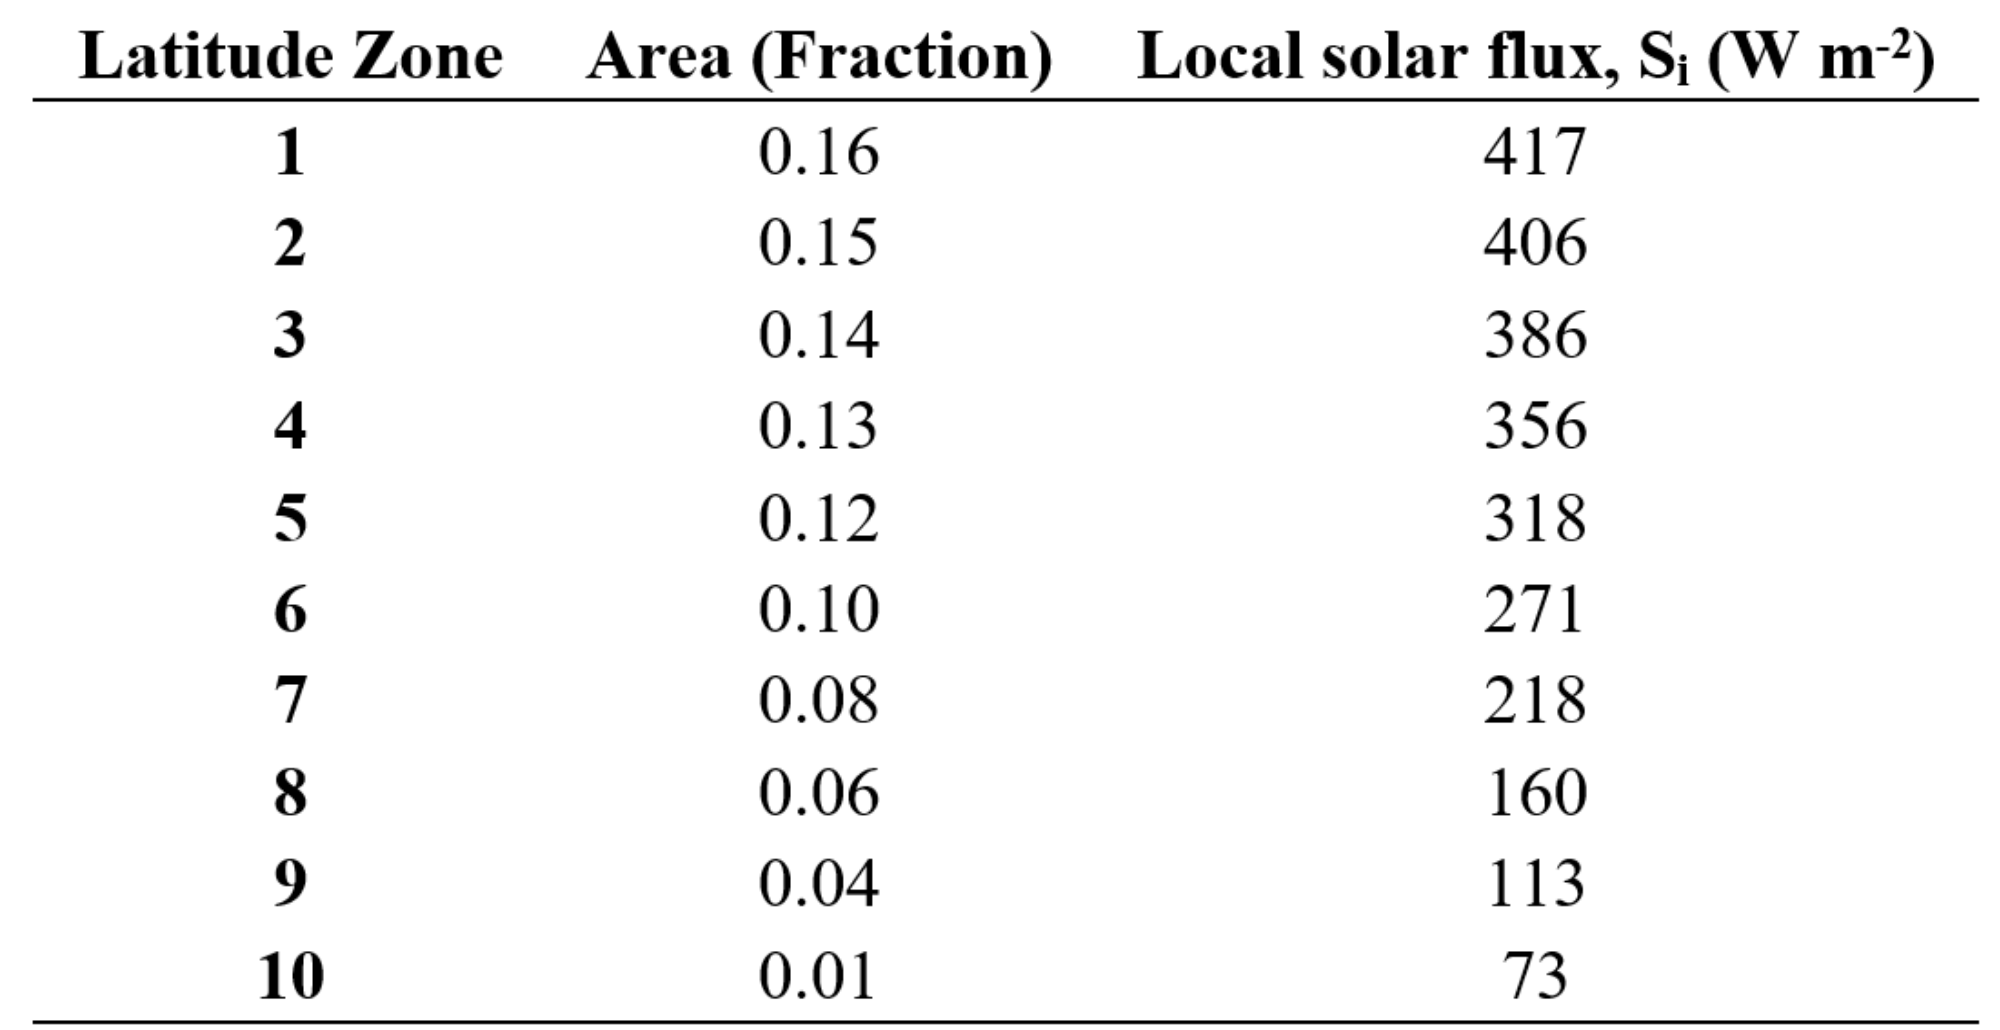
\includegraphics[width=1\textwidth,height=\textheight]{Media/Table5.png}

}

\end{figure}

Use the zonal insolation data (\(S_i\)) to calculate \(F_{gain}\) at
each latitude band.

\begin{equation}
\tag{8}
F_{gain} = S_i * (1-\alpha_i) * M
\end{equation}

\hypertarget{b-temperature}{%
\subparagraph{(B) Temperature}\label{b-temperature}}

Let's define the average planet temperature as:

\begin{equation}
\tag{9}
T_{avg} = \sum(area_i * T_i)
\end{equation}

\hypertarget{c-energy-loss-from-earth}{%
\subparagraph{(C) Energy loss from
Earth}\label{c-energy-loss-from-earth}}

The energy emitted/lost at each latitude band is given by the local
temperature (\(T_i\)) and the average temperature (\(T_{avg}\)):

\begin{equation}
\tag{10}
F_{loss} = A + B * T_i + G * (T_i - T_{avg})
\end{equation}

G represents heat transfer coefficient. \(F_{loss}\) at each latitude
band is then calculated.

\hypertarget{local-and-average-albedo}{%
\paragraph{8.3 LOCAL AND AVERAGE
ALBEDO}\label{local-and-average-albedo}}

Let's now find the local albedo (\(\alpha_i\)). At each latitude band,
the albedo is fixed at 0.3 (current Earth's albedo) when the temperature
is \(\ge -10^\circ\)C (critical T), otherwise it is 0.6 (ice albedo).
The same way as the temperature, the average albedo of the planet is the
sum of the area-weighted albedos.

\begin{equation}
\tag{11}
\alpha_{average} = \sum(area_i * \alpha_i)
\end{equation}

\hypertarget{equilibrium-states}{%
\paragraph{8.4 EQUILIBRIUM STATES}\label{equilibrium-states}}

Our objective is to find the equilibrium average temperature of the
planet for a specific solar luminosity (\(T_{eq}\) against \(M\)). In
other words, how does the planet's temperature change when the overall
solar energy received changes.

You'll need to find the average temperature (T) at equilibrium for the
values of the solar multiplier (\(M\)) going from 0.6 to 1.4. First, run
the model by increasing \(M\) (0.6 to 1.4) and then by decreasing \(M\)
(1.4 to 0.6). Collect the equilibrium temperature for each solar
multiplier.

\[F_{loss} = A + B * T_i + G * (T_i - T_{avg})\]
\[F_{gain} = S_i * (1-\alpha_i) * M\]

At equilibrium, \(F_{gain} = F_{loss}\)

\[F_{gain} = F_{loss} = A + B * T_i + G * (T_i - T_{avg})\]

\begin{equation}
\tag{12}
T_i = \frac{F_{gain} - A + G * T_{avg}}{(B+G)}
\end{equation}

To find the equilibrium average planet temperature (\(T_{avg}\)), you
will start with an arbitrary condition (i.e.~local temperature for each
latitude band) and use the iteration method.

\hypertarget{initial-conditions}{%
\paragraph{8.5 INITIAL CONDITIONS}\label{initial-conditions}}

The solar constant is \(S_0 * M\) with \(M\) ranging from 0.6 to 1.4.

You will assume that it is the same initial temperature (\(T_i\) = 255K)
at each latitude band (with \(M\) = 0.6). Therefore, all local albedos
at the initial stage is equivalent to 0.6 (Earth is covered in ice).

\begin{tcolorbox}[enhanced jigsaw, titlerule=0mm, title={Modelling Questions}, arc=.35mm, breakable, colback=white, toprule=.15mm, colframe=quarto-callout-caution-color-frame, opacityback=0, bottomtitle=1mm, coltitle=black, toptitle=1mm, rightrule=.15mm, colbacktitle=quarto-callout-caution-color!10!white, bottomrule=.15mm, opacitybacktitle=0.6, leftrule=.75mm, left=2mm]

Let's construct a code to understand the ice-albedo model.

You are given two arrays containing the area of each band and its local
solar flux:

\begin{verbatim}
# Array containing area of each band and its local solar flux
Area = np.array([0.156434465, 0.152582529, 0.144973505, 0.133794753, 0.119321529, 0.101910213, 0.08198953, 0.060049992, 0.036631824, 0.012311659])
S    = np.array([416.6480383, 406.3887808, 386.1228828, 356.349358, 317.8013293, 271.4279772, 218.3711674, 160.4091221, 112.7543514, 73.14499959])

# Constants:
G, A, B = 3.8, 204, 2.17
\end{verbatim}

\textbf{M9.} Initialize two arrays to store the modelled Earth's bands
of temperatures (\emph{T\_0}) and albedos(\emph{albedo\_0}). \emph{Have
the planet first be -70\(^\circ\)C throughout.}

\textbf{Remember:} The critical temperature is \(-10^\circ\)C, albedo is
0.3 \(\ge -10^\circ\)C and albedo is 0.6 \(\le -10^\circ\)C.

\begin{center}\rule{0.5\linewidth}{0.5pt}\end{center}

\textbf{M10.} Understand and complete the flowchart of the ice-albedo
model given below.
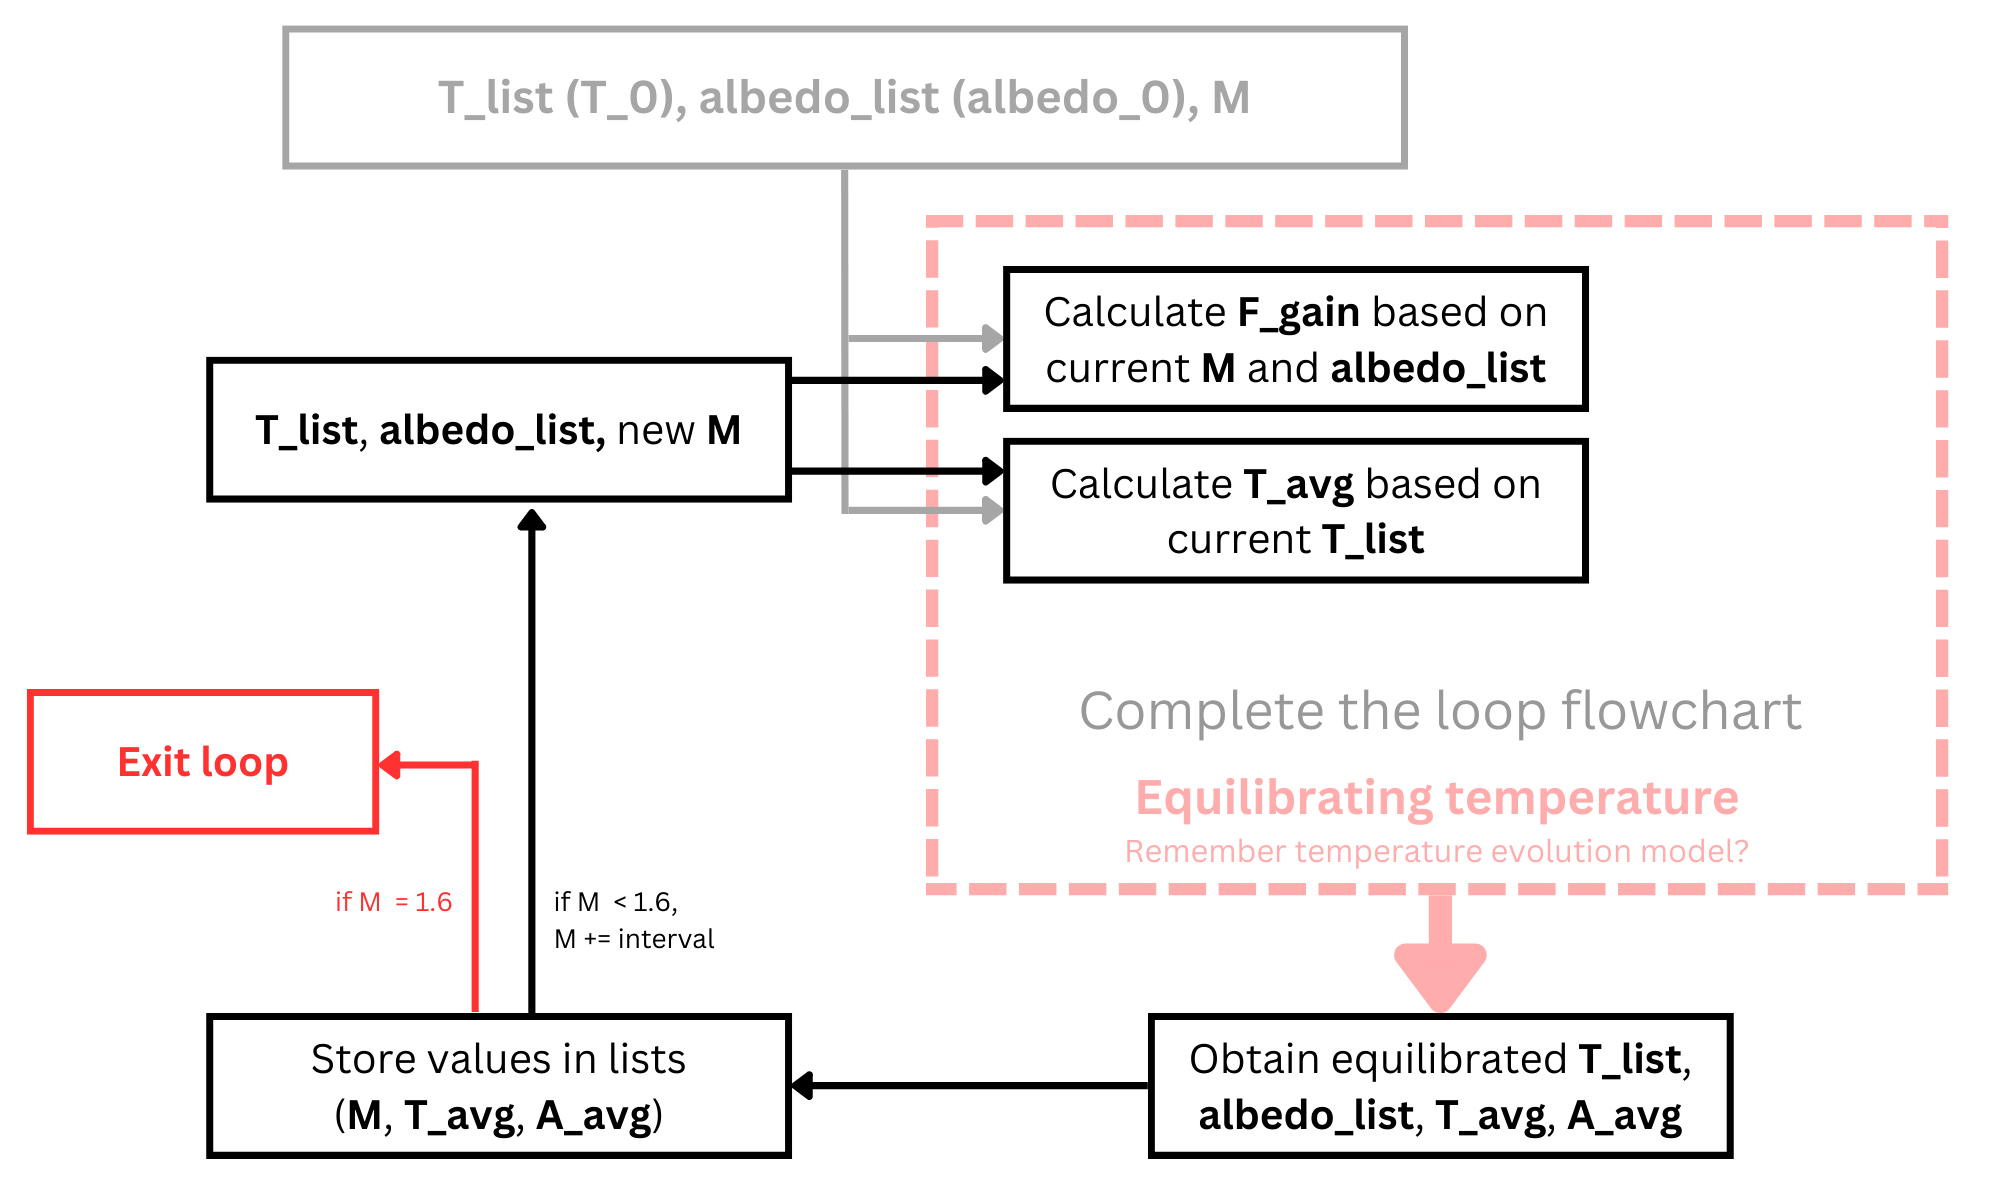
\includegraphics[width=1\textwidth,height=\textheight]{Media/FlowChart2.png}

\begin{center}\rule{0.5\linewidth}{0.5pt}\end{center}

\textbf{M11.} Based on the flowchart, construct the code to compute the
ice-albedo model and plot the graphs for increasing and decreasing solar
multiplier (\(M\)).

\end{tcolorbox}

\hypertarget{understanding-the-graph}{%
\paragraph{8.6 UNDERSTANDING THE GRAPH}\label{understanding-the-graph}}

The ice-albedo model aims to relate the concept of feedback cycles and
how they affect the surface temperature of the Earth to achieve
equilibrium. In \textbf{Exercise 7}, attempt to draw the feedback cycles
when surface temperatures drops or when it rises. You'll find that both
feedback cycles show a positive feedback loop which magnifies the
effects of the change in solar luminosity.

The ice-albedo model show how changes of the Earth's polar ice caps can
have huge effects on the entire planet's climate. For more information,
look into the supplementary materials on Earth's paleoclimate.

\subsubsection{\texorpdfstring{\textbf{Exercise 7}}{Exercise 7}}

Illustrate two positive feedback loops when \textbf{1.} surface
temperatures drops and \textbf{2.} when surface temperature rises
incorporating the below factors:

\begin{itemize}
\tightlist
\item
  Surface temperature
\item
  Ice Cover
\item
  Earth's albedo
\item
  \(F_{gain}\)
\end{itemize}

\subsubsection{\texorpdfstring{\textbf{Model Answer}}{Model Answer}}

\begin{figure}

{\centering 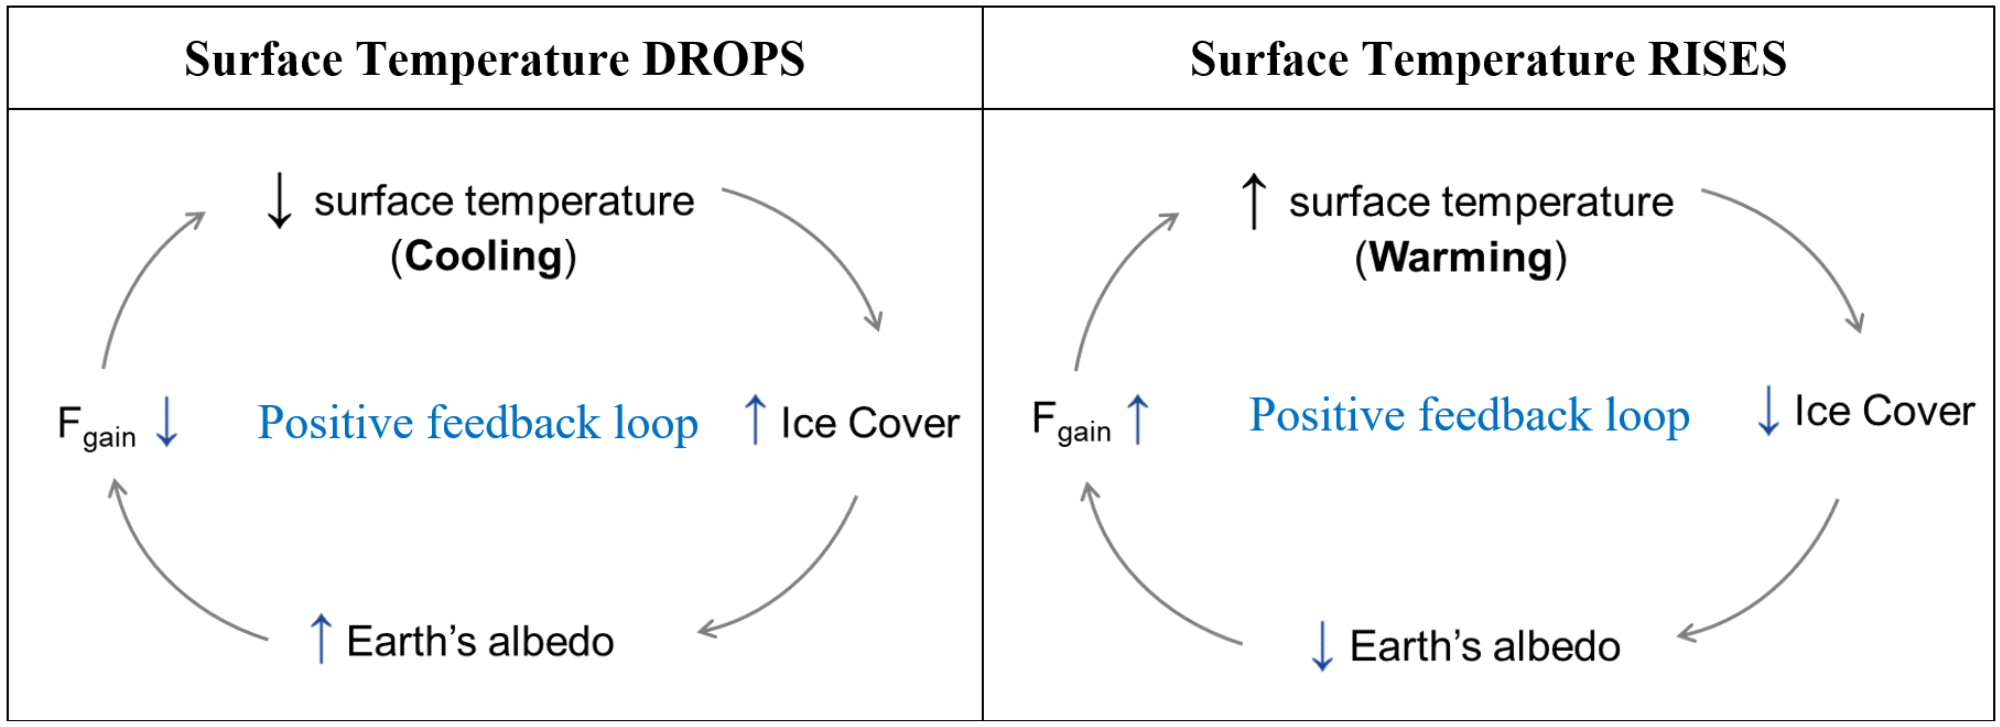
\includegraphics[width=1\textwidth,height=\textheight]{Media/Figure15.png}

}

\caption{\textbf{Figure 16:} Positive feedback loops of the Ice-albedo
model}

\end{figure}

However, why does the surface temperature trend go differently depending
on the increasing or decreasing of the solar luminosity? This phenomenon
is a hysteresis. Hysteresis is the dependence of the state of a system
on its initial conditions. So, how were the initial conditions different
that could help to explain the hysteresis observed in the graph plot of
equilibrium temperature against \(M\)?

\begin{quote}
\textbf{Discussion corner}

Why does the surface temperature trend go differently depending on the
increasing or decreasing of the solar luminosity?
\end{quote}

\hypertarget{deliverables}{%
\subsection{9 \textbar{} DELIVERABLES}\label{deliverables}}

\hypertarget{learning-flow}{%
\paragraph{Learning Flow}\label{learning-flow}}

Students are to complete the assigned work before their lecture and IS
sessions to ensure for a smooth and fruitful discussion session with
their groupmates and mentors. Minimum prepatory work for each session
has been labelled with ``*``.

\begin{figure}

{\centering 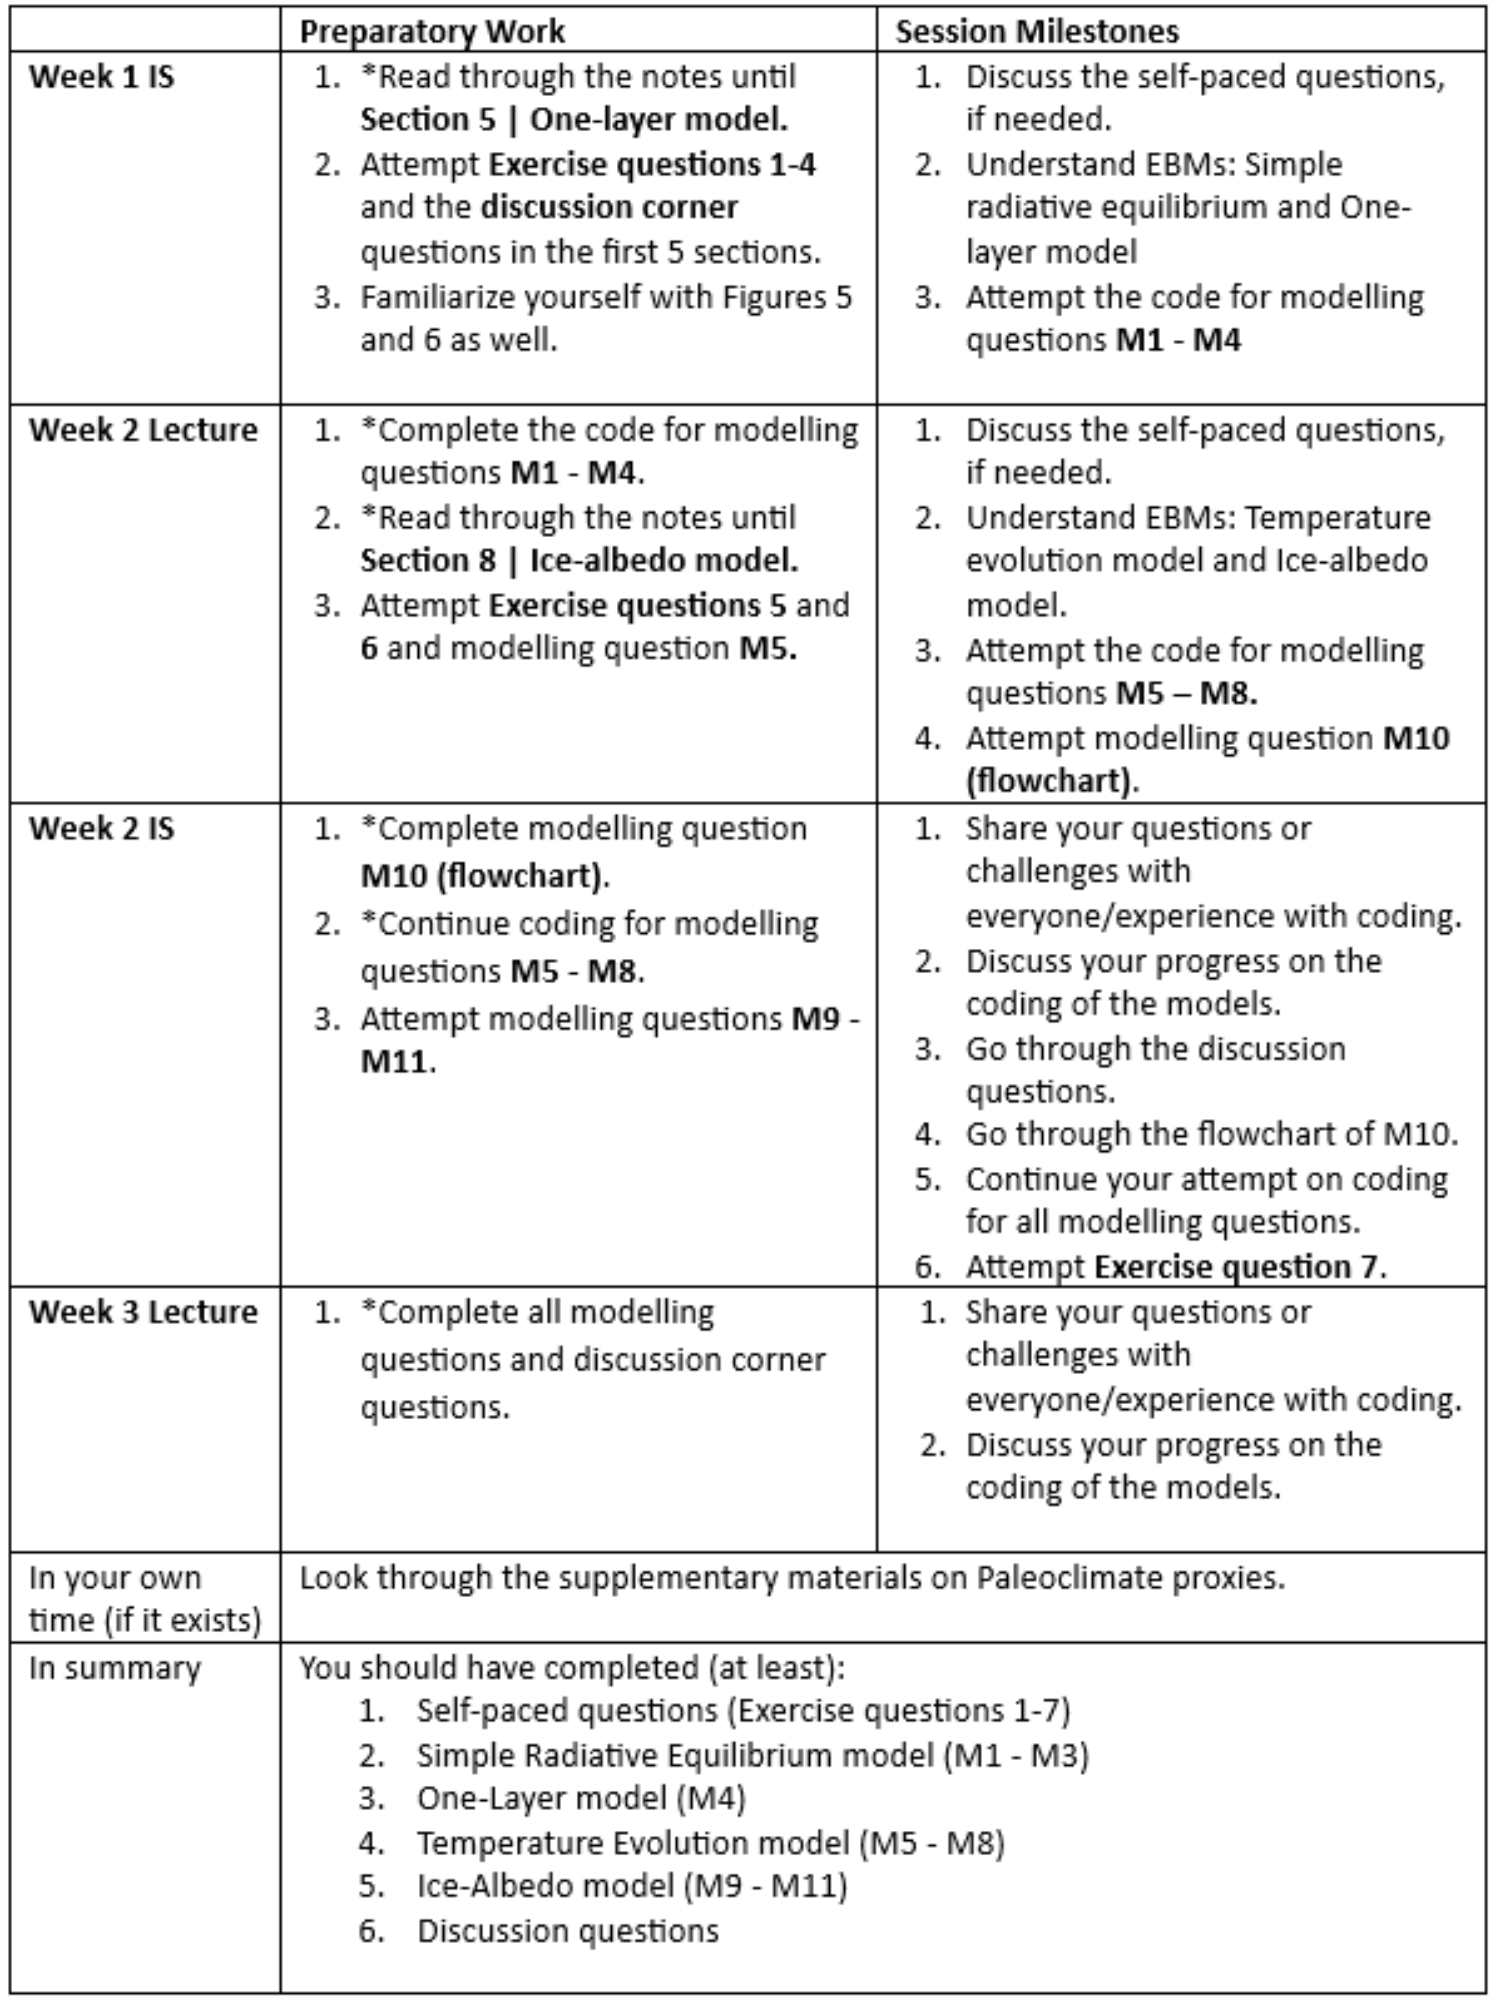
\includegraphics[width=0.8\textwidth,height=\textheight]{Media/Deliverables.png}

}

\end{figure}

\hypertarget{earth-journal}{%
\paragraph{Earth Journal}\label{earth-journal}}

(\emph{For the students concerned})

In your Earth Journal, summarize what are the key concepts and skills
you have acquired from this chapter and the significance of the topic.
In addition, you can write on the insights that you received from this
chapter and what questions you can ask yourself to learn further on the
topic. You can also write on how you can apply such knowledge to your
major.

\hypertarget{climate-presentation}{%
\paragraph{Climate Presentation}\label{climate-presentation}}

(\emph{For the groups concerned})

Prepare a presentation on what the class has learnt in this chapter. The
presentation should include the following elements:

\textbf{1.} Examine and discuss on the various energy balance models
learnt\\
\textbf{2.} Extensions on the topics learnt

Emphasize on the concepts and conclusions obtained from the codes
instead of presenting on how to code. Find ways to engage the class
better!

\hypertarget{references}{%
\subsection{10 \textbar{} REFERENCES}\label{references}}

Budyko, M. I. (1969). The effect of solar radiation variations on the
climate of the Earth. \emph{Tellus}, 21(5), 611-619.

Cess, R. D. (1976). Climate change: an appraisal of atmospheric feedback
mechanisms employing zonal climatology. \emph{Journal of atmospheric
sciences}, 33(10), 1831-1843.

Lenton, T. M., Rockström, J., Gaffney, O. et al.~(2019). Climate tipping
points -- too risky to bet against. \emph{Nature} 575, 592-595.
https://doi.org/10.1038/d41586-019-03595-0.

Lewis, S. (2020). How the atmosphere sustains life on Earth.
\emph{OpenLearn}. Retrieved June 23, 2022, from
https://www.open.edu/openlearn/science-maths-technology/across-the-sciences/how-the-atmosphere-sustains-life-on-earth.

McGuffie, K. \& Henderson-Sellers, A. (2005). \emph{A climate modelling
primer}. (3rd ed.) John Wiley \& Sons.
https://doi.org/10.1002/0470857617.

NASA (n.d.). Climate change: how do we know?. \emph{NASA Global Climate
Change: Vital Signs of the Planet}. Retrieved June 23, 2022, from
https://climate.nasa.gov/evidence/.

Sellers, W. D. (1969). A global climatic model based on the energy
balance of the Earth-atmosphere system. \emph{Journal of Applied
Meteorology}, 8(3), 392-400.

Tung, K. K. (2007). \emph{Topics in mathematical modeling}. Princeton
University Press.

Wilde, S., Valley, J., Peck, W. et al.~(2001). Evidence from detrital
zircons for the existence of continental crust and oceans on the Earth
4.4 Gyr ago. \emph{Nature} 409, 175-178.
https://doi.org/10.1038/35051550.

Wunderling, N., Donges, J. F., Kurths, J., Winkelmann, R. (2021).
Interacting tipping elements increase risk of climate domino effects
under global warming. \emph{Earth system dynamics}, 12, 601-619.
https://doi.org/10.5194/esd-12-601-2021.



\end{document}
